\documentclass[12pt]{extarticle}

%%%% paramètres généraux et commande prédéfinies
%%%% french character
\usepackage[french]{babel}
\usepackage[T1]{fontenc}
\usepackage[utf8]{inputenc}

%%%% useful packages
\usepackage[a4paper, left=1.3cm, right=1.3cm, top=2.2cm, bottom=2.3cm]{geometry}
\usepackage{subcaption} % for figure caption
\usepackage{graphicx} % image
\usepackage{tabularx} % table
\usepackage[table]{xcolor} % color in table
\usepackage{amsmath} % math
\usepackage{amssymb} % bold math
\usepackage{wasysym} % integral
\usepackage[many]{tcolorbox} % colored box
\usepackage{fancyhdr} % headers
\usepackage{enumitem} % for bullet in itemize
\usepackage[colorlinks=true,linkcolor=black,citecolor=black,filecolor=black,urlcolor=black]{hyperref} % for link
\usepackage{accents} % for complex notation
\usepackage[european, straightvoltages, RPvoltages]{circuitikz} % for electronic circuit
\usepackage{multicol} % to use several columns
\usepackage{fontawesome} % awesome icons
\usepackage{ifthen} % for loop and boolean in commands
\usepackage{pdfpages} % to include pdf
\usepackage{wrapfig} % to wrap text around figures
\usepackage{chemfig} % to draw chemistry formula
\usepackage{multirow} % for vertically merged cells
\usepackage{makecell} % to format cell in tables
\usepackage{physics} % for derivatives, braket, etc.
\usepackage{esvect} % for large vectors
\usepackage{listings} % for code
\usepackage{dashundergaps} % for automatic text to fill
\usepackage{tabularray} % for better tables
% dyslexia friendly font (need to be compiled in xetex)
%\usepackage{fontspec}
%\setmainfont{OpenDyslexic}


%%%% settings
\setlength{\parskip}{0cm}
\setlength{\parindent}{0cm}
\renewcommand{\baselinestretch}{1}
\setcounter{tocdepth}{2}


%%%% tikz configuration
\usetikzlibrary{babel}
\tikzset{>=latex}


%%%% header
\renewcommand{\headrulewidth}{0.4pt}
\setlength{\headheight}{22.50113pt}


%%%% Table
\renewcommand{\tabularxcolumn}[1]{m{#1}}
\setlength{\extrarowheight}{8pt}


%%%% Chemfig configuration
\setchemfig{
  atom sep=20pt,
  bond style={line width=1pt},
  angle increment=30
}


%%%% dashundergaps configuration
\dashundergapssetup{
  gap-numbers = false,
  gap-format = dot,
  gap-widen,
  gap-extend-percent
}

%%%% Mode élève (commenté) ou prof (décommenté)
%\modeCorrection
%%%% pour l'en-tête
\renewcommand{\annee}{2023-2024}
\renewcommand{\etablissement}{Lycée Jean Moulin}

%%%% TP
\begin{document}
  %%%% tube à essai de sang
\newcommand{\tubeEssaiSang}[1]{
  \begin{subfigure}{0.1\linewidth}
    \centering
    \begin{tikzpicture}
      \tkzBasTubeEssai{#1}{0.25}{0}{0.75}{0.1}
      \tkzTubeEssai{0.25}{1.5}{0.1}
    \end{tikzpicture}
    \caption{}
  \end{subfigure}
}

%%%% Tube à essai de sang centrifugé
\newcommand{\tubeEssaiSangC}[3]{
  \centering
  \begin{tikzpicture}
    \tkzBasTubeEssai{rougeSombre!75!white}{0.5}{0}{#1}{0.1}
    \tkzPhaseTubeEssai{gray!10!white}{0.5}{#1}{#2}{0.1}
    \tkzPhaseTubeEssai{jauneClair!75!white}{0.5}{#2}{#3}{0.1}
    \tkzLegende{Plasma}{0.5}{#3 - 0.5}{2}
    \tkzLegende{Globules blancs}{0.5}{#2-0.08}{2}
    \tkzLegende{Globules rouges}{0.5}{-0.1}{2}
    \tkzTubeEssai{0.5}{#3 + 1}{0.1}
  \end{tikzpicture}
  \caption{}
}


%%%%
\newcommand{\VEth}{V_\text{éth}}
\newcommand{\mEth}{m_\text{éth}}
\newcommand{\rhoEth}{\rho_\text{éth}}
\newcommand{\cEth}{c_\text{éth}}
\newcommand{\COeq}{kg\chemfig{CO_2}e\;}
  %%%% Sommative
  %% Seconde
  \sujetA
  %%%% début de la page
\teteSndCorp
\setcounter{page}{1}

%%%%
\nomPrenomClasse

%%%%
\titreEvaluation{\sndCorp}

%%%% Compétences évaluées
\sousTitre{Compétences évaluées}

\begin{tableauCompetences}
  \centering RCO &
  Connaître le vocabulaire du cours et les relations importantes.
  & & & & \\
  %
  \centering APP &
  Extraire des informations d'un document.
  & & & &  \\
  %
  \centering VAL &
  Comparer des valeurs calculées avec des valeurs de références pour valider un raisonnement.
  & & & & \\
  %
  \centering REA &
  Réaliser un calcul en donnant le résultat en notation scientifique avec les bonnes unités.
  & & & & \\
\end{tableauCompetences}

\appreciation{4}


%%%% Exercice I
\vspace*{-20pt}
\titrePartie{Marais salant et pollution}

Les marais salants sont de grands bassin remplis par d'eau de mer, qui est riche en sel.
Le sel est du chlorure de sodium de formule brute \chemfig{NaCl}.

%
\question{
  Indiquer en justifiant si l'eau de mer est un corps pur ou un mélange.\competence{RCO, APP}
}{
  C'est un mélange, composé d'au moins deux espèces chimique : l'eau et le sel.
}{1}

Le soleil et le vent font s'évaporer l'eau de mer, mais le sel reste au fond des bassins. 
Après plusieurs étapes d'évaporation et de remplissage, la quantité de sel contenue dans l'eau des bassins devient très importante.
La masse volumique de l'eau salée augmente avec la quantité de sel.

\question{
  Rappeler la relation mathématique entre la masse volumique de l'eau salée $\rho$, sa masse $m$ et le volume $V$ qu'elle occupe.\competence{RCO}
}{
  \begin{equation*}
    \rho = \frac{m}{V}
  \end{equation*}
}{2}

Les productrices ou producteurs peuvent récolter le sel lorsque la masse volumique de l'eau salée dans un bassin est \textbf{supérieure} à $\rho_\text{récolte} = \qty{1,15}{\g/\ml}$.

\question{
  Une productrice de sel pèse \qty{50}{\ml} d'eau salée provenant d'un bassin et mesure une masse de \variationSujet{\qty{60}{\g}}{\qty{55}{\g}}.
  Calculer la masse volumique de l'eau salée dans ce bassin.\competence{REA}
}{
  $m_\text{eau salée} = \qty{60}{\g}$ et $V_\text{eau salée} = \qty{50}{\ml}$. Donc 
  \begin{equation*}
    \rho_\text{eau salée} = \frac{\qty{60}{\g}}{\qty{50}{\ml}} = \qty{1,2}{\g/\ml}
  \end{equation*}
}{2}

\question{
  Est-ce que la productrice peut récolter le sel dans ce bassin ? Justifier.\competence{VAL}
}{
  La masse volumique de l'eau du bassin est \variationSujet{supérieure}{inférieure} à celle nécessaire pour récolter, donc la productrice \variationSujet{peut}{ne peut pas} récolter le sel.
}{2}


Une ingénieure agronome réalise une inspection des marais salants en baie de somme.
Pour vérifier que des ions ne pollue pas les marais, elle prélève puis teste l'eau des bassins avec différentes espèces chimiques.
Un tableau récapitulatif des tests qu'elle peut réaliser est présenté ci-dessous

\begin{center}
  \begin{tableau}{| c | c | c |}
    Espèce utilisée & Ion recherché & Résultat d'un test positif \\
    Nitrate d'argent & \ionChlorure & Précipité blanc \\
    \SetCell[r = 3]{c} Hydroxyde de sodium & \ionCuivreII & Précipité bleu \\
    & \ionFerII & Précipité vert \\
    & \ionFerIII & Précipité rouille \\
    Chlorure de baryum & \ionSulfate & Précipité blanc \\
  \end{tableau}
\end{center}

\question{
  L'ingénieure commence par verser quelques gouttes de \variationSujet{chlorure de Baryum}{nitrate d'argent} dans un tube à essai contenant l'eau prélevée.
  Elle observe la formation d'un précipité blanc.
  Indiquer quel ion pollue le bassin, en justifiant.\competence{APP}
}{
   D'après le tableau, le \variationSujet{chlorure de baryum}{nitrate d'argent} a réagit avec les ions \variationSujet{sulfates}{chlorure} pour former un précipité blanc.
}{2}

\question{
  L'ingénieure veut réaliser des tests supplémentaires pour savoir si le bassin est aussi pollué par des ions Fer.
  Indiquer quel(s) réactif(s) elle doit utiliser et quel résultat permettrait de conclure à la présence d'ions Fer.\competence{APP}
}{
  Pour identifier la présence d'ions fer, l'ingénieure devra réaliser un test avec l'hydroxyde de sodium.
  Si elle voit apparaître un précipité vert, alors le bassin contient des ions Fer II.
  Si elle voit apparaître un précipité rouille, alors le bassin contient des ions Fer III.
  Si aucun précipité n'apparaît, le bassin n'est pas pollué.
}{4}


%%%% Exercice II
\vspace*{-20pt}
\titrePartie{Huile essentielle de \variationSujet{lavande}{menthe}}

Les huiles essentielles de \variationSujet{lavande}{menthe} sont obtenues par distillation des fleurs de \variationSujet{lavandes}{menthe}.
Les huiles essentielles sont riches en molécules odorantes.
On réalise une Chromatographie sur Couche Mince (CCM) afin d'identifier quelques espèces chimiques présentes dans cette huile essentielle.
Le chromatogramme obtenue après la montée de l'éluant est présenté ci-dessous.

\begin{figure}[!ht]
  \centering
  \variationSujet{
    \image{0.21}{images/chromato_lavande}
  }{
    \image{0.2}{images/chromato_menthe}
  }
  
  A : huile essentielle de \variationSujet{lavande}{menthe},
  B : \variationSujet{linalol}{menthol},
  C : \variationSujet{acétate de linalyle}{limonène}
  
  Chromatogramme.
\end{figure}

\numeroQuestion
Indiquer sur le chromatogramme où se trouvent la ligne de dépôt, la couche mince et le front de l'éluant.\competence{RCO}

\question{
  Justifier que l'huile essentielle de \variationSujet{lavande}{menthe} est un mélange.\competence{RCO, APP}
}{
  D'après le chromatogramme, le dépôt d'huile essentielle s'est divisé en trois tâches, c'est donc un mélange.
}{2}

\question{
  En comparant les hauteurs des tâches, indiquer quelles sont les espèces chimiques présentes dans l'huile essentielle de \variationSujet{lavande}{menthe}.\competence{RCO, APP, VAL}
}{
  Sur un chromatogramme, deux composés sont identiques s'ils sont montés à la même hauteur. 
  Sur le chromatogramme, on voit que la première tâche d'huile essentielle de \variationSujet{lavande}{menthe} est à la même hauteur que le \variationSujet{l'acétate de linalyle}{limonène} et que la seconde tâche est à la même hauteur que le \variationSujet{linalol}{menthol}.
  L'huile essentielle de \variationSujet{lavande}{menthe} est donc composée de \variationSujet{l'acétate de linalyle}{limonène} et de \variationSujet{linalol}{menthol}.
}{3}

\question{
  Peut-on identifier le troisième composé présent dans l'huile essentielle avec ce chromatogramme ?\competence{APP, VAL}
}{
  Non, car on n'a pas d'espèce chimique de référence pour comparer.
}{2}


%%%% Exercice III
\titrePartie{Étalon du kilogramme}

\begin{wrapfigure}[6]{r}{0.2\linewidth}
  \centering
  \vspace*{-40pt}
  \image{0.9}{images/standard_kilogram.jpg}
\end{wrapfigure}

Le kilogramme est l'unité de base de la masse dans le système international.
L'étalon qui \textbf{a servi à définir le kilogramme} jusqu'en mai 2019 est conservé par le Bureau International des Poids et Mesures (BIPM).
Ce prototype est un cylindre constitué d'un alliage de platine et d'iridium, de volume $V_\text{étalon} = \qty{47,191}{\cm\cubed}$ et de masse volumique $\rho_\text{étalon} = \qty{21,191}{\g/\cm\cubed}$.

\question{
  Sans calcul, indiquer la masse de l'étalon.\competence{APP}
}{
  L'étalon sert à définir le kilogramme.
  Sa masse est donc de \qty{1}{\kg} par définition.
}{1}

\question{
  Le prototype est composé de \qty{0,9}{\kg} de platine et de \qty{0,1}{\kg} d'iridium.
  Calculer la fraction massique de platine et d'iridium.\competence{REA, APP}
}{
  Pour le platine : $\qty{0,9}{\kg} / \qty{1}{\kg} = \qty{90}{\percent}$.
  Pour l'iridium : $\qty{0,1}{\kg} / \qty{1}{\kg} = \qty{10}{\percent}$
}{2}

\textit{Rappel :} la fraction massique d'une espèce dans un échantillon est la masse de l'espèce divisée par la masse totale de l'échantillon.
Par exemple pour le platine :
\begin{equation*}
  p_v(\text{platine}) = \frac{m_\text{platine}}{m_\text{étalon}}
\end{equation*}

\question{
  Historiquement, un premier cylindre avait été réalisé avec \qty{11,1}{\percent} d'iridium, qui a une masse volumique plus élevée que le platine.
  Sachant que son volume était identique à l'étalon actuel, indiquer si la masse de ce cylindre valait 1 kg et expliquer pourquoi il avait été rejeté par le BIPM.\competence{APP}
}{
  L'étalon actuel a précisément une masse de \qty{1}{\kg} avec \qty{10}{\percent} d'iridium.
  Le premier cylindre comportait $\qty{11,1}{\percent} > \qty{10}{\percent}$ d'iridium.
  Comme l'iridium a une masse volumique plus élevée, sa masse valait plus de \qty{1}{\kg}, d'où le rejet par le BIPM.
}{2}


\setcounter{sousSectionNum}{0}

%%%% Correction
\newpage
\vspace*{-36pt}
\titreSousSection{Ma correction (à faire après la correction du professeur)}

%%%% Tableau de correction élève
\begin{tblr}{
    row{1} = {couleurPrim!20}, hlines,
    colspec = {| X[-1, c] | X[2, c] | X[2, c] | X[2, c] |}
  }
  \textbf{Question} & 
  \textbf{L'erreur} &
  \textbf{Analyse de l'erreur} &
  \textbf{La correction} \\
  %
  \phantom{b} \vspace{55 pt} & & & \\
  \phantom{b} \vspace{55 pt} & & & \\
  \phantom{b} \vspace{55 pt} & & & \\
  \phantom{b} \vspace{55 pt} & & & \\
\end{tblr}


%%%% Bilan
\titreSousSection{Mon bilan après mon travail de correction}

%%%% Tableau bilan de la correction
\begin{tableau}{| X[c] | X[c] |}
  \textbf{Ce que je n'avais pas compris...} &
  \textbf{Ce que maintenant j'ai compris...} \\
  \phantom{b} \vspace{150 pt} & \\
\end{tableau}


%%%% Acquis
\titreSousSection{Mes acquis après mon travail de correction (à remplir par le professeur)}

\appreciation{2}
  \sujetB
  %%%% début de la page
\teteSndCorp
\setcounter{page}{1}

%%%%
\nomPrenomClasse

%%%%
\titreEvaluation{\sndCorp}

%%%% Compétences évaluées
\sousTitre{Compétences évaluées}

\begin{tableauCompetences}
  \centering RCO &
  Connaître le vocabulaire du cours et les relations importantes.
  & & & & \\
  %
  \centering APP &
  Extraire des informations d'un document.
  & & & &  \\
  %
  \centering VAL &
  Comparer des valeurs calculées avec des valeurs de références pour valider un raisonnement.
  & & & & \\
  %
  \centering REA &
  Réaliser un calcul en donnant le résultat en notation scientifique avec les bonnes unités.
  & & & & \\
\end{tableauCompetences}

\appreciation{4}


%%%% Exercice I
\vspace*{-20pt}
\titrePartie{Marais salant et pollution}

Les marais salants sont de grands bassin remplis par d'eau de mer, qui est riche en sel.
Le sel est du chlorure de sodium de formule brute \chemfig{NaCl}.

%
\question{
  Indiquer en justifiant si l'eau de mer est un corps pur ou un mélange.\competence{RCO, APP}
}{
  C'est un mélange, composé d'au moins deux espèces chimique : l'eau et le sel.
}{1}

Le soleil et le vent font s'évaporer l'eau de mer, mais le sel reste au fond des bassins. 
Après plusieurs étapes d'évaporation et de remplissage, la quantité de sel contenue dans l'eau des bassins devient très importante.
La masse volumique de l'eau salée augmente avec la quantité de sel.

\question{
  Rappeler la relation mathématique entre la masse volumique de l'eau salée $\rho$, sa masse $m$ et le volume $V$ qu'elle occupe.\competence{RCO}
}{
  \begin{equation*}
    \rho = \frac{m}{V}
  \end{equation*}
}{2}

Les productrices ou producteurs peuvent récolter le sel lorsque la masse volumique de l'eau salée dans un bassin est \textbf{supérieure} à $\rho_\text{récolte} = \qty{1,15}{\g/\ml}$.

\question{
  Une productrice de sel pèse \qty{50}{\ml} d'eau salée provenant d'un bassin et mesure une masse de \variationSujet{\qty{60}{\g}}{\qty{55}{\g}}.
  Calculer la masse volumique de l'eau salée dans ce bassin.\competence{REA}
}{
  $m_\text{eau salée} = \qty{60}{\g}$ et $V_\text{eau salée} = \qty{50}{\ml}$. Donc 
  \begin{equation*}
    \rho_\text{eau salée} = \frac{\qty{60}{\g}}{\qty{50}{\ml}} = \qty{1,2}{\g/\ml}
  \end{equation*}
}{2}

\question{
  Est-ce que la productrice peut récolter le sel dans ce bassin ? Justifier.\competence{VAL}
}{
  La masse volumique de l'eau du bassin est \variationSujet{supérieure}{inférieure} à celle nécessaire pour récolter, donc la productrice \variationSujet{peut}{ne peut pas} récolter le sel.
}{2}


Une ingénieure agronome réalise une inspection des marais salants en baie de somme.
Pour vérifier que des ions ne pollue pas les marais, elle prélève puis teste l'eau des bassins avec différentes espèces chimiques.
Un tableau récapitulatif des tests qu'elle peut réaliser est présenté ci-dessous

\begin{center}
  \begin{tableau}{| c | c | c |}
    Espèce utilisée & Ion recherché & Résultat d'un test positif \\
    Nitrate d'argent & \ionChlorure & Précipité blanc \\
    \SetCell[r = 3]{c} Hydroxyde de sodium & \ionCuivreII & Précipité bleu \\
    & \ionFerII & Précipité vert \\
    & \ionFerIII & Précipité rouille \\
    Chlorure de baryum & \ionSulfate & Précipité blanc \\
  \end{tableau}
\end{center}

\question{
  L'ingénieure commence par verser quelques gouttes de \variationSujet{chlorure de Baryum}{nitrate d'argent} dans un tube à essai contenant l'eau prélevée.
  Elle observe la formation d'un précipité blanc.
  Indiquer quel ion pollue le bassin, en justifiant.\competence{APP}
}{
   D'après le tableau, le \variationSujet{chlorure de baryum}{nitrate d'argent} a réagit avec les ions \variationSujet{sulfates}{chlorure} pour former un précipité blanc.
}{2}

\question{
  L'ingénieure veut réaliser des tests supplémentaires pour savoir si le bassin est aussi pollué par des ions Fer.
  Indiquer quel(s) réactif(s) elle doit utiliser et quel résultat permettrait de conclure à la présence d'ions Fer.\competence{APP}
}{
  Pour identifier la présence d'ions fer, l'ingénieure devra réaliser un test avec l'hydroxyde de sodium.
  Si elle voit apparaître un précipité vert, alors le bassin contient des ions Fer II.
  Si elle voit apparaître un précipité rouille, alors le bassin contient des ions Fer III.
  Si aucun précipité n'apparaît, le bassin n'est pas pollué.
}{4}


%%%% Exercice II
\vspace*{-20pt}
\titrePartie{Huile essentielle de \variationSujet{lavande}{menthe}}

Les huiles essentielles de \variationSujet{lavande}{menthe} sont obtenues par distillation des fleurs de \variationSujet{lavandes}{menthe}.
Les huiles essentielles sont riches en molécules odorantes.
On réalise une Chromatographie sur Couche Mince (CCM) afin d'identifier quelques espèces chimiques présentes dans cette huile essentielle.
Le chromatogramme obtenue après la montée de l'éluant est présenté ci-dessous.

\begin{figure}[!ht]
  \centering
  \variationSujet{
    \image{0.21}{images/chromato_lavande}
  }{
    \image{0.2}{images/chromato_menthe}
  }
  
  A : huile essentielle de \variationSujet{lavande}{menthe},
  B : \variationSujet{linalol}{menthol},
  C : \variationSujet{acétate de linalyle}{limonène}
  
  Chromatogramme.
\end{figure}

\numeroQuestion
Indiquer sur le chromatogramme où se trouvent la ligne de dépôt, la couche mince et le front de l'éluant.\competence{RCO}

\question{
  Justifier que l'huile essentielle de \variationSujet{lavande}{menthe} est un mélange.\competence{RCO, APP}
}{
  D'après le chromatogramme, le dépôt d'huile essentielle s'est divisé en trois tâches, c'est donc un mélange.
}{2}

\question{
  En comparant les hauteurs des tâches, indiquer quelles sont les espèces chimiques présentes dans l'huile essentielle de \variationSujet{lavande}{menthe}.\competence{RCO, APP, VAL}
}{
  Sur un chromatogramme, deux composés sont identiques s'ils sont montés à la même hauteur. 
  Sur le chromatogramme, on voit que la première tâche d'huile essentielle de \variationSujet{lavande}{menthe} est à la même hauteur que le \variationSujet{l'acétate de linalyle}{limonène} et que la seconde tâche est à la même hauteur que le \variationSujet{linalol}{menthol}.
  L'huile essentielle de \variationSujet{lavande}{menthe} est donc composée de \variationSujet{l'acétate de linalyle}{limonène} et de \variationSujet{linalol}{menthol}.
}{3}

\question{
  Peut-on identifier le troisième composé présent dans l'huile essentielle avec ce chromatogramme ?\competence{APP, VAL}
}{
  Non, car on n'a pas d'espèce chimique de référence pour comparer.
}{2}


%%%% Exercice III
\titrePartie{Étalon du kilogramme}

\begin{wrapfigure}[6]{r}{0.2\linewidth}
  \centering
  \vspace*{-40pt}
  \image{0.9}{images/standard_kilogram.jpg}
\end{wrapfigure}

Le kilogramme est l'unité de base de la masse dans le système international.
L'étalon qui \textbf{a servi à définir le kilogramme} jusqu'en mai 2019 est conservé par le Bureau International des Poids et Mesures (BIPM).
Ce prototype est un cylindre constitué d'un alliage de platine et d'iridium, de volume $V_\text{étalon} = \qty{47,191}{\cm\cubed}$ et de masse volumique $\rho_\text{étalon} = \qty{21,191}{\g/\cm\cubed}$.

\question{
  Sans calcul, indiquer la masse de l'étalon.\competence{APP}
}{
  L'étalon sert à définir le kilogramme.
  Sa masse est donc de \qty{1}{\kg} par définition.
}{1}

\question{
  Le prototype est composé de \qty{0,9}{\kg} de platine et de \qty{0,1}{\kg} d'iridium.
  Calculer la fraction massique de platine et d'iridium.\competence{REA, APP}
}{
  Pour le platine : $\qty{0,9}{\kg} / \qty{1}{\kg} = \qty{90}{\percent}$.
  Pour l'iridium : $\qty{0,1}{\kg} / \qty{1}{\kg} = \qty{10}{\percent}$
}{2}

\textit{Rappel :} la fraction massique d'une espèce dans un échantillon est la masse de l'espèce divisée par la masse totale de l'échantillon.
Par exemple pour le platine :
\begin{equation*}
  p_v(\text{platine}) = \frac{m_\text{platine}}{m_\text{étalon}}
\end{equation*}

\question{
  Historiquement, un premier cylindre avait été réalisé avec \qty{11,1}{\percent} d'iridium, qui a une masse volumique plus élevée que le platine.
  Sachant que son volume était identique à l'étalon actuel, indiquer si la masse de ce cylindre valait 1 kg et expliquer pourquoi il avait été rejeté par le BIPM.\competence{APP}
}{
  L'étalon actuel a précisément une masse de \qty{1}{\kg} avec \qty{10}{\percent} d'iridium.
  Le premier cylindre comportait $\qty{11,1}{\percent} > \qty{10}{\percent}$ d'iridium.
  Comme l'iridium a une masse volumique plus élevée, sa masse valait plus de \qty{1}{\kg}, d'où le rejet par le BIPM.
}{2}


\setcounter{sousSectionNum}{0}

%%%% Correction
\newpage
\vspace*{-36pt}
\titreSousSection{Ma correction (à faire après la correction du professeur)}

%%%% Tableau de correction élève
\begin{tblr}{
    row{1} = {couleurPrim!20}, hlines,
    colspec = {| X[-1, c] | X[2, c] | X[2, c] | X[2, c] |}
  }
  \textbf{Question} & 
  \textbf{L'erreur} &
  \textbf{Analyse de l'erreur} &
  \textbf{La correction} \\
  %
  \phantom{b} \vspace{55 pt} & & & \\
  \phantom{b} \vspace{55 pt} & & & \\
  \phantom{b} \vspace{55 pt} & & & \\
  \phantom{b} \vspace{55 pt} & & & \\
\end{tblr}


%%%% Bilan
\titreSousSection{Mon bilan après mon travail de correction}

%%%% Tableau bilan de la correction
\begin{tableau}{| X[c] | X[c] |}
  \textbf{Ce que je n'avais pas compris...} &
  \textbf{Ce que maintenant j'ai compris...} \\
  \phantom{b} \vspace{150 pt} & \\
\end{tableau}


%%%% Acquis
\titreSousSection{Mes acquis après mon travail de correction (à remplir par le professeur)}

\appreciation{2}
  % \sujetA
  % %%%% début de la page
\newpage
\setcounter{page}{1}
\sndEnTeteUn

%%%%
\nomPrenomClasse

%%%%
\numeroActivite{2}
\vspace*{-8pt}
\titreEvaluation{Solutions}

%%%% evaluation
\sousTitre{\large Compétences évaluées}
\vspace*{6pt}

\competenceEvaluationDeux

\appreciation{120}

%%%% Exercice 2
\titrePartie{Sang et anémie}

Le sang est un mélange liquide composé de $54 \%$ de plasma, $45 \%$ de globules rouges et $1 \%$ de globules blancs.
On peut séparer ses constituants en utilisant une centrifugeuse, ce qui donnerait un mélange constitué de trois phases, comme présenté figure~\ref{fig:sang}.

%
\question{
  Indiquer en justifiant si le contenu des tubes à essais de la figure~\ref{fig:sang} est un mélange homogène ou un mélange hétérogènes.\competence{RCO, APP}
}{
  ...
}{0}


Le plasma est une solution aqueuse, qui contient des minéraux, des nutriments et les gaz lié à la respiration (dioxygène \chemfig{O_2} et dioxyde de carbone \chemfig{CO_2}).

%
\question{
  Indiquer le solvant et les solutés qui constituent le plasma.\competence{RCO}
}{
  ...
}{0}


Pour assurer son bon fonctionnement, l'organisme d'un être humain a besoin de fer \chemfig{Fe}.
On dit qu'une personne souffre d'anémie si la concentration massique en fer dans le sang est trop faible.
Le fer est transporté par une molécule dans le sang : l'hémoglobine.

\begin{figure}[!ht]
  \centering
  %
  \begin{subfigure}{0.48\linewidth}
    \tubeEssaiSangC{1.3}{1.4}{2.5}
    \label{fig:sang_normal}
  \end{subfigure}
  %
  \begin{subfigure}{0.48\linewidth}
    \tubeEssaiSangC{0.45}{0.55}{2.5}
    \label{fig:sang_anemie}
  \end{subfigure}
  %
  \caption{
    \centering
    Tube à essai contenant un échantillon de sang centrifugé : (a) d'une personne normale ; (b) d'une personne souffrant d'anémie.
  }
  \label{fig:sang}
\end{figure}

%
\question{
  En utilisant la figure~\ref{fig:sang}, indiquer en justifiant quel constituant du sang contient les molécules d'hémoglobines.\competence{APP, ANA/RAI}
}{
  ...
}{0}
\newpage


Mesurer la concentration massique en hémoglobine dans le sang permet de détecter les cas d'anémies.
On parle d'anémie si cette concentration massiques est inférieure a $1,\!2 \unit{g/L}$ pour une femme et $1,\!3 \unit{g/L}$ pour un homme.
Pour mesurer cette concentration, on peut réaliser une échelle de teinte, car c'est l'hémoglobine qui donne sa teinte rouge au sang.

\begin{figure}[!ht]
  %
  \centering
  \tubeEssaiSang{rougeClair}
  \tubeEssaiSang{rougeClair!75!white}
  \tubeEssaiSang{rougeClair!50!white}
  \tubeEssaiSang{rougeClair!25!white}
  \tubeEssaiSang{rougeClair!10!white} \\[4pt]
  \begin{subfigure}{0.6\linewidth}
    \centering
    \setlength{\extrarowheight}{4pt}
    \begin{tabular}{c | c | c | c | c | c}
      \rowcolor{gray!15} Solution & a   & b   & c   & d   & e \\ \hline
      Concentration (g/L)         & 1,4 & 1,3 & 1,2 & 1,1 & 1,0
    \end{tabular}
    \caption{}
  \end{subfigure}
  \tubeEssaiSang{rougeClair!65!white}
  %
  \caption{Schéma de l'échelle de teinte réalisée, avec les solutions étalons (a, b, c, d, e), leurs concentrations (f) et l'échantillon de sang à doser (g).}
  \label{fig:echelle_teinte}
\end{figure}

%
\question{
  Rappeler avec vos mots le principe général d'un dosage par étalonnage (que veut-on mesurer et comment fait-on).\competence{RCO, COM}
}{
  ...
}{0}

%
\question{
  Pour préparer des solutions, on peut effectuer une dilution ou une dissolution. Indiquer en justifiant laquelle des deux on effectue pour passer de la solution (a) à la solution (b).\competence{RCO, APP}
}{
  ...
}{0}
  
%
\question{
  Donner le nom de deux verreries nécessaires pour réaliser une dilution.\competence{RCO}
}{
  ...
}{0}

%
\question{
  En utilisant la figure~\ref{fig:echelle_teinte}, indiquer en justifiant la concentration en hémoglobine de l'échantillon de sang (g).\competence{APP, ANA/RAI, VAL}
}{
  ...
}{0}

%
\question{
  L'échantillon vient \variationSujet{d'une femme}{d'un homme}. Indiquer en justifiant si \variationSujet{elle}{il} souffre d'anémie ou non.\competence{APP, ANA/RAI, VAL}
}{
  ...
}{0}


%%%% Exercice 1
\newpage
\vspace*{-8pt}
\titrePartie{Conduite et alcoolémie}

Mélanie et sa femme Sihame sortent en voiture pour aller manger dehors.
Au restaurant Sihame boit un verre de \variationSujet{$200 \unit{mL}$}{$250 \unit{mL}$} d'alcool à $10 \degree$ : c'est-à-dire que $10 \%$ du volume de la boisson est de l'éthanol.

On va chercher à déterminer si Sihame pourra de nouveau conduire après le repas.

%
\question{
  Calculer le volume d'éthanol dans le verre.\competence{APP, REA}
}{
  ...
}{0}

%
\question{
  Sachant que l'éthanol a une masse volumique qui vaut $\rho_\text{éth} = 0,\!8 \unit{g/mL}$ et que $m_\text{éth} = \rho_\text{éth} \times V_\text{éth}$, calculer la masse d'éthanol bue par Sihame.\competence{APP, REA}
}{
  ...
}{0}


Le corps d'une femme adulte contient en moyenne $4,\!5 \unit{L}$ de sang. En France, \og \textit{il est interdit de conduire avec un taux d'alcool dans le sang supérieur ou égal à $0,5 \unit{g/l}$ de sang} \fg.

%
\question{
  Indiquer le nom de la grandeur utilisé en physique-chimie pour désigner le taux d'alcool dans le sang. Expliquer avec vos mots la différence entre cette grandeur et la masse volumique.\competence{RCO, COM}
}{
  ...
}{0}

%
\question{
  Rappeler la formule de la concentration massique.\competence{RCO}
}{
  ...
}{0}

%
\question{
  Calculer la concentration massique d'éthanol dans le sang de Sihame.\competence{APP, REA}
}{
  ...
}{0}

%
\question{
  Indiquer, en justifiant, si Sihame pourra conduire en sortant du restaurant.\competence{APP, VAl, ANA/RAI, COM}
}{
  ...
}{0}


En fait, quand un humain boit une boisson alcoolisé seule une petite partie de l'éthanol et absorbé par l'organisme. En moyenne seulement $12\%$ de l'éthanol passe dans le sang (si on a bu $10\unit{g}$ d'éthanol, $1,\!2\unit{g}$ passe dans le sang).

%
\question{
  Calculer de nouveau la concentration massique dans le sang de Sihame en tenant compte de cette information. Indiquer, en justifiant, si Sihame pourra conduire en sortant du restaurant.\competence{APP, REA, VAL, ANA/RAI, COM}
}{
  ...
}{0}

\setcounter{sousSection}{0}

%%%% Correction
\newpage
\vspace*{-36pt}
\titreSousSection{Ma correction (à faire après la correction du professeur)}

\correctionEleve{40}


%%%% Bilan
\titreSousSection{Mon bilan après mon travail de correction}

\bilanCorrection{125}


%%%% Acquis
\titreSousSection{Mes acquis après mon travail de correction (à remplir par le professeur)}

\appreciation{80}
  % \sujetB
  % %%%% début de la page
\newpage
\setcounter{page}{1}
\sndEnTeteUn

%%%%
\nomPrenomClasse

%%%%
\numeroActivite{2}
\vspace*{-8pt}
\titreEvaluation{Solutions}

%%%% evaluation
\sousTitre{\large Compétences évaluées}
\vspace*{6pt}

\competenceEvaluationDeux

\appreciation{120}

%%%% Exercice 2
\titrePartie{Sang et anémie}

Le sang est un mélange liquide composé de $54 \%$ de plasma, $45 \%$ de globules rouges et $1 \%$ de globules blancs.
On peut séparer ses constituants en utilisant une centrifugeuse, ce qui donnerait un mélange constitué de trois phases, comme présenté figure~\ref{fig:sang}.

%
\question{
  Indiquer en justifiant si le contenu des tubes à essais de la figure~\ref{fig:sang} est un mélange homogène ou un mélange hétérogènes.\competence{RCO, APP}
}{
  ...
}{0}


Le plasma est une solution aqueuse, qui contient des minéraux, des nutriments et les gaz lié à la respiration (dioxygène \chemfig{O_2} et dioxyde de carbone \chemfig{CO_2}).

%
\question{
  Indiquer le solvant et les solutés qui constituent le plasma.\competence{RCO}
}{
  ...
}{0}


Pour assurer son bon fonctionnement, l'organisme d'un être humain a besoin de fer \chemfig{Fe}.
On dit qu'une personne souffre d'anémie si la concentration massique en fer dans le sang est trop faible.
Le fer est transporté par une molécule dans le sang : l'hémoglobine.

\begin{figure}[!ht]
  \centering
  %
  \begin{subfigure}{0.48\linewidth}
    \tubeEssaiSangC{1.3}{1.4}{2.5}
    \label{fig:sang_normal}
  \end{subfigure}
  %
  \begin{subfigure}{0.48\linewidth}
    \tubeEssaiSangC{0.45}{0.55}{2.5}
    \label{fig:sang_anemie}
  \end{subfigure}
  %
  \caption{
    \centering
    Tube à essai contenant un échantillon de sang centrifugé : (a) d'une personne normale ; (b) d'une personne souffrant d'anémie.
  }
  \label{fig:sang}
\end{figure}

%
\question{
  En utilisant la figure~\ref{fig:sang}, indiquer en justifiant quel constituant du sang contient les molécules d'hémoglobines.\competence{APP, ANA/RAI}
}{
  ...
}{0}
\newpage


Mesurer la concentration massique en hémoglobine dans le sang permet de détecter les cas d'anémies.
On parle d'anémie si cette concentration massiques est inférieure a $1,\!2 \unit{g/L}$ pour une femme et $1,\!3 \unit{g/L}$ pour un homme.
Pour mesurer cette concentration, on peut réaliser une échelle de teinte, car c'est l'hémoglobine qui donne sa teinte rouge au sang.

\begin{figure}[!ht]
  %
  \centering
  \tubeEssaiSang{rougeClair}
  \tubeEssaiSang{rougeClair!75!white}
  \tubeEssaiSang{rougeClair!50!white}
  \tubeEssaiSang{rougeClair!25!white}
  \tubeEssaiSang{rougeClair!10!white} \\[4pt]
  \begin{subfigure}{0.6\linewidth}
    \centering
    \setlength{\extrarowheight}{4pt}
    \begin{tabular}{c | c | c | c | c | c}
      \rowcolor{gray!15} Solution & a   & b   & c   & d   & e \\ \hline
      Concentration (g/L)         & 1,4 & 1,3 & 1,2 & 1,1 & 1,0
    \end{tabular}
    \caption{}
  \end{subfigure}
  \tubeEssaiSang{rougeClair!65!white}
  %
  \caption{Schéma de l'échelle de teinte réalisée, avec les solutions étalons (a, b, c, d, e), leurs concentrations (f) et l'échantillon de sang à doser (g).}
  \label{fig:echelle_teinte}
\end{figure}

%
\question{
  Rappeler avec vos mots le principe général d'un dosage par étalonnage (que veut-on mesurer et comment fait-on).\competence{RCO, COM}
}{
  ...
}{0}

%
\question{
  Pour préparer des solutions, on peut effectuer une dilution ou une dissolution. Indiquer en justifiant laquelle des deux on effectue pour passer de la solution (a) à la solution (b).\competence{RCO, APP}
}{
  ...
}{0}
  
%
\question{
  Donner le nom de deux verreries nécessaires pour réaliser une dilution.\competence{RCO}
}{
  ...
}{0}

%
\question{
  En utilisant la figure~\ref{fig:echelle_teinte}, indiquer en justifiant la concentration en hémoglobine de l'échantillon de sang (g).\competence{APP, ANA/RAI, VAL}
}{
  ...
}{0}

%
\question{
  L'échantillon vient \variationSujet{d'une femme}{d'un homme}. Indiquer en justifiant si \variationSujet{elle}{il} souffre d'anémie ou non.\competence{APP, ANA/RAI, VAL}
}{
  ...
}{0}


%%%% Exercice 1
\newpage
\vspace*{-8pt}
\titrePartie{Conduite et alcoolémie}

Mélanie et sa femme Sihame sortent en voiture pour aller manger dehors.
Au restaurant Sihame boit un verre de \variationSujet{$200 \unit{mL}$}{$250 \unit{mL}$} d'alcool à $10 \degree$ : c'est-à-dire que $10 \%$ du volume de la boisson est de l'éthanol.

On va chercher à déterminer si Sihame pourra de nouveau conduire après le repas.

%
\question{
  Calculer le volume d'éthanol dans le verre.\competence{APP, REA}
}{
  ...
}{0}

%
\question{
  Sachant que l'éthanol a une masse volumique qui vaut $\rho_\text{éth} = 0,\!8 \unit{g/mL}$ et que $m_\text{éth} = \rho_\text{éth} \times V_\text{éth}$, calculer la masse d'éthanol bue par Sihame.\competence{APP, REA}
}{
  ...
}{0}


Le corps d'une femme adulte contient en moyenne $4,\!5 \unit{L}$ de sang. En France, \og \textit{il est interdit de conduire avec un taux d'alcool dans le sang supérieur ou égal à $0,5 \unit{g/l}$ de sang} \fg.

%
\question{
  Indiquer le nom de la grandeur utilisé en physique-chimie pour désigner le taux d'alcool dans le sang. Expliquer avec vos mots la différence entre cette grandeur et la masse volumique.\competence{RCO, COM}
}{
  ...
}{0}

%
\question{
  Rappeler la formule de la concentration massique.\competence{RCO}
}{
  ...
}{0}

%
\question{
  Calculer la concentration massique d'éthanol dans le sang de Sihame.\competence{APP, REA}
}{
  ...
}{0}

%
\question{
  Indiquer, en justifiant, si Sihame pourra conduire en sortant du restaurant.\competence{APP, VAl, ANA/RAI, COM}
}{
  ...
}{0}


En fait, quand un humain boit une boisson alcoolisé seule une petite partie de l'éthanol et absorbé par l'organisme. En moyenne seulement $12\%$ de l'éthanol passe dans le sang (si on a bu $10\unit{g}$ d'éthanol, $1,\!2\unit{g}$ passe dans le sang).

%
\question{
  Calculer de nouveau la concentration massique dans le sang de Sihame en tenant compte de cette information. Indiquer, en justifiant, si Sihame pourra conduire en sortant du restaurant.\competence{APP, REA, VAL, ANA/RAI, COM}
}{
  ...
}{0}

\setcounter{sousSection}{0}

%%%% Correction
\newpage
\vspace*{-36pt}
\titreSousSection{Ma correction (à faire après la correction du professeur)}

\correctionEleve{40}


%%%% Bilan
\titreSousSection{Mon bilan après mon travail de correction}

\bilanCorrection{125}


%%%% Acquis
\titreSousSection{Mes acquis après mon travail de correction (à remplir par le professeur)}

\appreciation{80}
  % sommative 3
  % %%%% début de la page
\newpage
\setcounter{page}{1}
\sndEnTeteDeux

%%%%
\nomPrenomClasse

%%%%
\numeroActivite{3}
\titreEvaluation{\sndChapitreDeux}

%%%% evaluation
\sousTitre{\large Compétences évaluées}
\vspace*{6pt}

\competenceEvaluationTrois

\appreciation{90}

%%%%
\vspace*{-24pt}
\titrePartie{Impesanteur}

%%
\vspace*{-4pt}
\begin{doc}{Station spatiale internationale (ISS)}
  On lit parfois que les spationautes flottent dans les stations spatiales, car la gravité terrestre n'agit plus sur les spationautes.

  \begin{wrapfigure}{r}{0.4\linewidth}
    \vspace*{-32pt}
    \centering
    \image{0.9}{sommative/2nd_Mouv/spationaute_ISS}
  \end{wrapfigure}
  
  On s'intéresse à la station spatiale internationale (ou ISS), en orbite circulaire autour de la Terre à une hauteur $h$. L'ISS a une vitesse constante $v$.

  \textbf{Données :}
  \begin{listePoints}
    \item $G = 6,\!67 \times 10^{-11} \unit{N \cdot m^2 \cdot kg^{-2}}$
    \item $\MTerre = 5,\!97 \times 10^{24} \unit{kg}$
    \item $\RTerre = 6,\!37 \times 10^3 \unit{km}$
    \item $h = 3,\!70 \times 10^2 \unit{km}$
    \item $v = 7,\!66 \times 10^3 \unit{m\cdot s^{-1}}$
  \end{listePoints}
\end{doc}

%%
\vspace*{-24pt}
\question{
  \label{exo:schema_ISS}
  Quel est le mouvement décrit par l'ISS dans le référentiel lié au centre de la Terre ?
  Faire un schéma faisant figurer l'ISS, la Terre et la trajectoire qu'elle décrit.\competence{APP}
}{0}

\question{
  Dans la station les spationautes ont un poids $P = m \times \gISS$.
  Calculer la valeur de $\gISS = G \times \Frac{\MTerre}{(\RTerre + h)^2}$.\competence{APP, REA}
}{0}

\question{
  Comparer avec l'accélération de pesanteur terrestre $g = 9,\!81 \unit{N\cdot kg^{-1}}$.
  Peut-on vraiment dire que la gravité terrestre n'agit plus sur les spationautes au sein de l'ISS ?\competence{VAL, ANA/RAI}
}{0}

\question{
  \label{exo:calcul_poids_ISS}
  En sachant que $\gISS = 8,\!77 \unit{N\cdot kg^{-1}}$, calculer le poids d'une spationaute de masse $m = 65 \unit{kg}$ dans l'ISS.\competence{REA}
}{0}

%%
\begin{doc}{Force d'inertie d'entraînement}
  Un système dans un référentiel en rotation est soumis à une force \textit{relative} (qui dépend du référentiel), qu'on appelle \textbf{force d'inertie d'entraînement} $\vv{F}_\inertie$ ou encore \og force centrifuge \fg.

  Cette force a pour direction la droite reliant le centre du cercle et le centre du système.
  Son sens est dirigé vers l'extérieur du cercle.
  C'est cette force qui explique pourquoi les passagers d'une voiture dans un rond-point sentent leur corps attiré vers l'extérieur du rond-point.
\end{doc}

\question{
  Expliquer avec vos mot le principe d'inertie.\competence{RCO, COM}
}{0}

\question{
  Dans le référentiel lié à l'ISS, cette spationaute est immobile.
  En utilisant le principe d'inertie et en justifiant clairement, donner la norme de la force d'inertie d'entraînement $F_\inertie$ qui s'exerce sur la spationaute.\competence{RCO, APP, ANA/RAI}
}{0}

\question{
  Compléter le schéma de la question~\ref{exo:schema_ISS} en représentant les forces s'exerçant sur la spationaute dans le référentiel lié à l'ISS.\competence{APP, REA}
}{0}

\question{
  La norme de la force d'inertie d'entraînement exercée sur la spationaute est
  \begin{equation}
    F_\inertie = m \times \frac{v^2}{R}
    \label{eq:force_inertie}
  \end{equation}
  où $v$ est la vitesse du référentiel et $R$ est la distance entre le centre de rotation du référentiel et le centre du système. 
  Cette relation est-elle cohérente avec le principe d'inertie ?
  
  \textit{
    Prendre des initiatives et les écrire, même si le raisonnement n'est pas complet.
    Tout début de réflexion sera valorisé.
  }
  \competence{APP, REA, VAL, ANA/RAI}
}{0}

%% Formulation officielle du BAC
% Le candidat est invité à prendre des initiatives et à présenter la démarche suivie, même si elle n'a pas abouti. La démarche est évaluée et nécessite d'être correctement présentée.

\begin{coupDePouce}
  Utiliser les données de l'énoncé pour calculer la norme de la force d'inertie d'entraînement avec la relation~(\ref{eq:force_inertie}). 
  Comparer cette norme avec celle obtenue à la question~\ref{exo:calcul_poids_ISS} et conclure.
\end{coupDePouce}


%%%%
\vspace*{-48pt}
\titrePartie{Mouvement d'un ballon}

%%
\vspace*{-8pt}
\begin{doc}{Penalty}
  Lors du match France-Angleterre de la coupe du monde masculine de football de 2022, un joueur anglais a tiré et raté un penalty.
  On s'intéresse au mouvement du ballon avant, puis pendant le tir du penalty.
\end{doc}

%%
\question{
  Avant le tir le ballon est immobile sur le sol. Lister les forces qui s'exercent sur le ballon. Schématiser le ballon et les forces qui s'exercent sur lui.\competence{RCO, APP, REA, ANA/RAI}
}{0}

\question{
  Les forces qui s'exercent sur le ballon se compensent-elles ?\competence{RCO, APP, ANA/RAI}
}{0}

%%
\vspace*{-8pt}
\begin{doc}{Chronophotographie}
  \label{doc:mouvement_ballon}
  Votre professeur préféré a réalisé une chronophotographie de la position du centre du ballon pendant le tir. \textbf{La durée entre chaque image est $\mathbf{\Delta t = 0,\!018 \unit{s}}$.} ($t_1 = 0\unit{s}$, $t_2 = \Delta t$, $t_3 = 2\times \Delta t, \ldots$)
  \begin{center}
    \image{0.7}{sommative/2nd_Mouv/penalty}
    
    \small{
      Position du ballon (en mètre)
    }
  \end{center}
\end{doc}

\question{
  Pendant le tir, quel référentiel permet d'étudier le mouvement du ballon ? (Donner un objet de référence.)\competence{RCO, APP, ANA/RAI}
}{0}

\question{
  \label{exo:mvt_ballon}
  D'après la chronophotographie du document~\ref{doc:mouvement_ballon}, décrire le mouvement du ballon, en justifiant.\competence{RCO, APP}
}{0}

\question{
  Calculer la norme des vecteurs vitesses $\vv{v}_2$ et $\vv{v}_6$.\competence{RCO, APP, REA}
}{0}

% \begin{coupDePouce}
%   Commencer par calculer la distance parcourue entre les points $P_1$ et $P_3$ pour $v_2$ (ou $P_5$ et $P_7$ pour $v_6$).
% \end{coupDePouce}

\question{
  Tracer sur le bas du document~\ref{doc:mouvement_ballon} les vecteurs vitesses $\vv{v}_2$ et $\vv{v}_6$ en choisissant une échelle pertinente.\competence{REA, ANA/RAI}
}{0}

\question{
  Pendant un penalty, en moyenne les ballons tirés ont une vitesse $v = 150\unit{km \cdot h^{-1}}$.
  Discuter du réalisme des données de l'énoncé. \textbf{Rappel :} $1 \unit{m\cdot s^{-1}} = 3,\!6 \unit{km\cdot h^{-1}}$ \competence{REA, VAL, ANA/RAI}
}{0}


\setcounter{sousSection}{0}

%%%% Correction
\newpage
\vspace*{-36pt}
\titreSousSection{Ma correction (à faire après la correction du professeur)}

\correctionEleve{40}


%%%% Bilan
\titreSousSection{Mon bilan après mon travail de correction}

\bilanCorrection{125}


%%%% Acquis
\titreSousSection{Mes acquis après mon travail de correction (à remplir par le professeur)}

\appreciation{80}
  % %%%% début de la page
\newpage
\setcounter{page}{1}
\sndEnTeteDeux

%%%%
\nomPrenomClasse

%%%%
\numeroActivite{3}
\titreEvaluation{\sndChapitreDeux}

%%%% evaluation
\sousTitre{\large Compétences évaluées}
\vspace*{6pt}

\competenceEvaluationTrois

\appreciation{90}

%%%%
\vspace*{-24pt}
\titrePartie{Impesanteur}

%%
\vspace*{-4pt}
\begin{doc}{Station spatiale internationale (ISS)}
  On lit parfois que les spationautes flottent dans les stations spatiales, car la gravité terrestre n'agit plus sur les spationautes.

  \begin{wrapfigure}{r}{0.4\linewidth}
    \vspace*{-32pt}
    \centering
    \image{0.9}{sommative/2nd_Mouv/spationaute_ISS}
  \end{wrapfigure}
  
  On s'intéresse à la station spatiale internationale (ou ISS), en orbite circulaire autour de la Terre à une hauteur $h$. L'ISS a une vitesse constante $v$.

  \textbf{Données :}
  \begin{listePoints}
    \item $G = 6,\!67 \times 10^{-11} \unit{N \cdot m^2 \cdot kg^{-2}}$
    \item $\MTerre = 5,\!97 \times 10^{24} \unit{kg}$
    \item $\RTerre = 6,\!37 \times 10^3 \unit{km}$
    \item $h = 3,\!70 \times 10^2 \unit{km}$
    \item $v = 7,\!66 \times 10^3 \unit{m\cdot s^{-1}}$
  \end{listePoints}
\end{doc}

%%
\vspace*{-24pt}
\question{
  \label{exo:schema_ISS}
  Quel est le mouvement décrit par l'ISS dans le référentiel lié au centre de la Terre ?
  Faire un schéma faisant figurer l'ISS, la Terre et la trajectoire qu'elle décrit.\competence{APP}
}{0}

\question{
  Dans la station les spationautes ont un poids $P = m \times \gISS$.
  Calculer la valeur de $\gISS = G \times \Frac{\MTerre}{(\RTerre + h)^2}$.\competence{APP, REA}
}{0}

\question{
  Comparer avec l'accélération de pesanteur terrestre $g = 9,\!81 \unit{N\cdot kg^{-1}}$.
  Peut-on vraiment dire que la gravité terrestre n'agit plus sur les spationautes au sein de l'ISS ?\competence{VAL, ANA/RAI}
}{0}

\question{
  \label{exo:calcul_poids_ISS}
  En sachant que $\gISS = 8,\!77 \unit{N\cdot kg^{-1}}$, calculer le poids d'une spationaute de masse $m = 70 \unit{kg}$ dans l'ISS.\competence{REA}
}{0}

%%
\begin{doc}{Force d'inertie d'entraînement}
  Un système dans un référentiel en rotation est soumis à une force \textit{relative} (qui dépend du référentiel), qu'on appelle \textbf{force d'inertie d'entraînement} $\vv{F}_\inertie$ ou encore \og force centrifuge \fg.

  Cette force a pour direction la droite reliant le centre du cercle et le centre du système.
  Son sens est dirigé vers l'extérieur du cercle.
  C'est cette force qui explique pourquoi les passagers d'une voiture dans un rond-point sentent leur corps attiré vers l'extérieur du rond-point.
\end{doc}

\question{
  Expliquer avec vos mot le principe d'inertie.\competence{RCO, COM}
}{0}

\question{
  Dans le référentiel lié à l'ISS, cette spationaute est immobile.
  En utilisant le principe d'inertie et en justifiant clairement, donner la norme de la force d'inertie d'entraînement $F_\inertie$ qui s'exerce sur la spationaute.\competence{RCO, APP, ANA/RAI}
}{0}

\question{
  Compléter le schéma de la question~\ref{exo:schema_ISS} en représentant les forces s'exerçant sur la spationaute dans le référentiel lié à l'ISS.\competence{APP, REA}
}{0}

\question{
  La norme de la force d'inertie d'entraînement exercée sur la spationaute est
  \begin{equation}
    F_\inertie = m \times \frac{v^2}{R}
    \label{eq:force_inertie}
  \end{equation}
  où $v$ est la vitesse du référentiel et $R$ est la distance entre le centre de rotation du référentiel et le centre du système. 
  Cette relation est-elle cohérente avec le principe d'inertie ?
  
  \textit{
    Prendre des initiatives et les écrire, même si le raisonnement n'est pas complet.
    Tout début de réflexion sera valorisé.
  }
  \competence{APP, REA, VAL, ANA/RAI}
}{0}

%% Formulation officielle du BAC
% Le candidat est invité à prendre des initiatives et à présenter la démarche suivie, même si elle n'a pas abouti. La démarche est évaluée et nécessite d'être correctement présentée.

\begin{coupDePouce}
  Utiliser les données de l'énoncé pour calculer la norme de la force d'inertie d'entraînement avec la relation~(\ref{eq:force_inertie}). 
  Comparer cette norme avec celle obtenue à la question~\ref{exo:calcul_poids_ISS} et conclure.
\end{coupDePouce}


%%%%
\vspace*{-48pt}
\titrePartie{Mouvement d'un ballon}

%%
\vspace*{-8pt}
\begin{doc}{Penalty}
  Lors du match France-Angleterre de la coupe du monde masculine de football de 2022, un joueur anglais a tiré et raté un penalty.
  On s'intéresse au mouvement du ballon avant, puis pendant le tir du penalty.
\end{doc}

%%
\question{
  Avant le tir le ballon est immobile sur le sol. Lister les forces qui s'exercent sur le ballon. Schématiser le ballon et les forces qui s'exercent sur lui.\competence{RCO, APP, REA, ANA/RAI}
}{0}

\question{
  Les forces qui s'exercent sur le ballon se compensent-elles ?\competence{RCO, APP, ANA/RAI}
}{0}

%%
\vspace*{-8pt}
\begin{doc}{Chronophotographie}
  \label{doc:mouvement_ballon}
  Votre professeur préféré a réalisé une chronophotographie de la position du centre du ballon pendant le tir. \textbf{La durée entre chaque image est $\mathbf{\Delta t = 0,\!052 \unit{s}}$.} ($t_1 = 0\unit{s}$, $t_2 = \Delta t$, $t_3 = 2\times \Delta t, \ldots$)
  \begin{center}
    \image{0.7}{sommative/2nd_Mouv/penalty}
    
    \small{
      Position du ballon (en mètre)
    }
  \end{center}
\end{doc}

\question{
  Pendant le tir, quel référentiel permet d'étudier le mouvement du ballon ? (Donner un objet de référence.)\competence{RCO, APP, ANA/RAI}
}{0}

\question{
  \label{exo:mvt_ballon}
  D'après la chronophotographie du document~\ref{doc:mouvement_ballon}, décrire le mouvement du ballon, en justifiant.\competence{RCO, APP}
}{0}

\question{
  Calculer la norme des vecteurs vitesses $\vv{v}_2$ et $\vv{v}_6$.\competence{RCO, APP, REA}
}{0}

% \begin{coupDePouce}
%   Commencer par calculer la distance parcourue entre les points $P_1$ et $P_3$ pour $v_2$ (ou $P_5$ et $P_7$ pour $v_6$).
% \end{coupDePouce}

\question{
  Tracer sur le bas du document~\ref{doc:mouvement_ballon} les vecteurs vitesses $\vv{v}_2$ et $\vv{v}_6$ en choisissant une échelle pertinente.\competence{REA, ANA/RAI}
}{0}

\question{
  Pendant un penalty, en moyenne les ballons tirés ont une vitesse $v = 150\unit{km \cdot h^{-1}}$.
  Discuter du réalisme des données de l'énoncé. \textbf{Rappel :} $1 \unit{m\cdot s^{-1}} = 3,\!6 \unit{km\cdot h^{-1}}$ \competence{REA, VAL, ANA/RAI}
}{0}

\setcounter{sousSection}{0}

%%%% Correction
\newpage
\vspace*{-36pt}
\titreSousSection{Ma correction (à faire après la correction du professeur)}

\correctionEleve{40}


%%%% Bilan
\titreSousSection{Mon bilan après mon travail de correction}

\bilanCorrection{125}


%%%% Acquis
\titreSousSection{Mes acquis après mon travail de correction (à remplir par le professeur)}

\appreciation{80}
  % sommative 4
  % \sujetA
  % %%%% début de la page
\newpage
\setcounter{page}{1}
\sndEnTeteTrois

%%%%
\nomPrenomClasse

%%%%
\numeroActivite{4}
\titreEvaluation{\sndChapitreTrois}

%%%% evaluation
\sousTitre{\large Compétences évaluées}
\vspace*{6pt}

\competenceEvaluationQuatre

\appreciation{90}

%%%%
\titreSection{Atome et élément chimique}

\numeroQuestion
  Dans la notation symbolique d'un atome \isotope{A}{Z}{X}
  \begin{listePoints}
    \item $Z$ est \texteTrouLigneComplete{le nombre de protons, appelé numéro atomique.}
    \item $A$ est \texteTrouLigneComplete{le nombre de nucléons, appelé nombre de masse.}
  \end{listePoints}

\question{
  \variationSujet
  {Dans les batteries on trouve du silicium \isotope{28}{14}{Si}.}
  {Le magnésium \isotope{25}{12}{Mg} est un réactif très présent en chimie.}
  Donner la composition du noyau de cet atome.\competence{APP, REA}
}{
  L'atome de silicium \isotope{28}{14}{Si} possède 14 protons et $28 - 14 = 14$ neutrons.
}{2}

\question{
  Indiquer en justifiant le nombre d'électrons que possède l'atome
  \variationSujet
  {de silicium.}
  {de magnésium.}
  \competence{APP, ANA/RAI}
}{
  L'atome est neutre électriquement, sa charge électrique totale est nulle.
  Les protons ont une charge positive, les électrons une charge négative.
  L'atome doit donc avoir autant de protons que d'électrons, soit 14 électrons.
}{2}

\question{
  La masse d'un électron est de l'ordre de $10^{-30} \unit{kg}$.
  Un proton est mille fois plus lourd.
  Donner l'ordre de grandeur de la masse d'un proton en kilogramme, en détaillant le calcul.\competence{REA, ANA/RAI}
}{
  $m_\text{proton} 
  = 1000 \times m_\text{électron} 
  = 10^3 \times 10^{-30} \unit{kg} 
  = 10^{-27} \unit{kg}$
}{3}


Certains élément chimiques peuvent exister sous plusieurs formes appelée isotope, comme par exemple
\variationSujet
{le carbone : \isotope{13}{6}{C}, \isotope{14}{6}{C}.}
{l'oxygène : \isotope{17}{8}{O}, \isotope{18}{8}{O}.}


\question{
  Le troisième isotope stable
  \variationSujet
  {du carbone possède 6 protons et 6 neutrons.}
  {de l'oxygène possède 8 protons et 8 neutrons.}
  Écrire sa représentation symbolique \isotope{A}{Z}{C}.\competence{REA}
}{
  L'atome de carbone a $6 + 6 = 12$ nucléons, on le note \isotope{12}{6}{C}.
}{1}

\question{
  Calculer la masse de l'atome
  \variationSujet
  {de carbone \isotope{13}{6}{C},}
  {d'oxygène \isotope{16}{8}{O},}
  en détaillant les calculs.\competence{APP, REA}
  
  \textbf{Données :} $m_\text{nucléon} = 1,\!67 \times 10^{-27} \unit{kg}$, $m_\text{électron} = 9,\!11 \times 10^{-31} \unit{kg}$
}{
  Les électrons étant 1000 fois plus léger que les nucléons, leurs masses est négligeable et la masse de l'atome est simplement le nombre de nucléons multiplié par la masse d'un nucléon
  \begin{equation*}
    m_{\chemfig{C}} 
    = 13 \times m_\text{nucléon} 
    = 13 \times 1,\!67 \cdot 10^{-27} \unit{kg}
    = 21,\!7 \cdot 10^{-27} \unit{kg}
  \end{equation*}
}{3}

\question{
  Le cuivre \isotope{63}{29}{Cu} peut devenir l'ion \chemfig{Cu^{2+}}.
  Donner le nombre de protons, neutrons et électrons de l'ion \chemfig{Cu^{2+}}. Justifier.\competence{APP, ANA/RAI}
}{
  L'ion \chemfig{Cu^{2+}} possède deux charges positives : 2 électrons ont donc été arrachés à l'atome de cuivre \isotope{63}{29}{Cu}.
  Cet atome possède 29 proton, $63 - 29 = 34$ neutrons et comme l'atome est neutre, il possède 29 électrons.
  L'ion \chemfig{Cu^{2+}} a donc 29 protons, 34 neutrons et $29 - 2 = 27$ électrons.
}{3}


%%%%
\titreSection{Ordre de grandeur et écologie}

On va chercher à estimer l'impact de notre alimentation sur le climat, en comparant avec l'impact du secteur automobile.
Pour cela on va estimer l'ordre de grandeur des émissions de gaz à effet de serre rejetés lors de la production de nos aliments.

Pour mesurer l'impact sur le climat d'un produit, on utilise le kilogramme de dioxyde de carbone équivalent (noté \COeq\!).
\textbf{Plus ce nombre est élevé et plus un produit a un impact important sur le dérèglement climatique.}

Par exemple, produire 1 kg de viande de mouton équivaut à l'émission de 39,72 kg de \chemfig{CO_2}, soit 39,72 \COeq (voir tableau).
Cette émission correspond à l'émission d'une voiture qui parcours 400 km.

\newpage
\vspace*{-30pt}
\question{
  Donner un ordre de grandeur du nombre de repas (déjeuner et dîner) par an. \textbf{Rappel :} 1 an = 365 jours\competence{REA}
}{
  Avec 2 repas par jour en moyenne, on a $2 \times 365 = 730 \sim 1000$ repas par an en ordre de grandeur.
}{1}

\question{
  \label{exo:ordre_alimentation}
  À l'aide du graphique ci-dessous, calculer en ordre de grandeur le \COeq annuel d'un régime à base de viande. On considère qu'un-e français-e mange en moyenne $0,\!1 \unit{kg}$ de viande par repas.\competence{APP, REA, ANA/RAI}
}{
  En ordre de grandeur, la production de $1\unit{kg}$ de mouton ou de poulet émet $10 \unit{\COeq}$.
  Par an, un-e français-e mange en moyenne $0,1 \unit{kg} \times 1000 = 100 \unit{kg}$ de viande par an.
  Par an, les émissions d'un-e français-e sera donc en moyenne les émissions pour $1\unit{kg}$ multipliée par la masse de viande mangée, soit
  \begin{equation*}
    100 \unit{kg} \times 10 \unit{\COeq / kg} = 10^3 \unit{\COeq}
  \end{equation*}
  On notera qu'un régime végétarien permet de diviser par 10 ses émissions liées à l'alimentation en ordre de grandeur !
}{3}

\begin{center}
  \vspace{-12pt}
  \image{0.75}{sommative/2nd_Atome/emission_CO2_alimentation}
\end{center}
\vspace{-12pt}

\question{
  %Une voiture à essence ou diesel émet en moyenne $0,\!1$ \COeq par km.
  %D'après le ministère de la transition écologique, une voiture parcoure en moyenne $12\, 200 \unit{km}$ par an.
  %Calculer l'ordre de grandeur des émissions de \COeq par an pour un-e français-e roulant en voiture.\competence{APP, REA, ANA/RAI}
  En moyenne, une personne qui possède une voiture en France émet $10^3$ \COeq en roulant \textbf{par an}.
  Comparer avec les émissions annuelle dues à l'alimentation.\competence{VAL}
}{
  On voit qu'en ordre de grandeur, les émissions liées à la voiture et à une alimentation à base de viande sont identiques.
}{2}

\question{
  En réalité, sur une année, le transport représente en moyenne $2,\!4 \times 10^3$ \COeq et l'alimentation $2,\!0 \times 10^3$ \COeq, sur un total annuel d'émission de $8,\!3 \times 10^3 $ \COeq pour une personne vivant en France.
  
  Le chiffre de l'alimentation est-il cohérent avec l'ordre de grandeur estimé question~\ref{exo:ordre_alimentation} ?\competence{APP, VAL}
}{
  En ordre de grandeur $2,\!0 \times 10^3 \unit{COeq} \sim 10^3 \unit{\COeq}$.
  Les estimations réalisées sont donc cohérentes avec les données mesurées.
}{2}

\setcounter{sousSection}{0}

%%%% Correction
\newpage
\vspace*{-36pt}
\titreSousSection{Ma correction (à faire après la correction du professeur)}

\correctionEleve{40}


%%%% Bilan
\titreSousSection{Mon bilan après mon travail de correction}

\bilanCorrection{125}


%%%% Acquis
\titreSousSection{Mes acquis après mon travail de correction (à remplir par le professeur)}

\appreciation{80}
  % \sujetB
  % %%%% début de la page
\newpage
\setcounter{page}{1}
\sndEnTeteTrois

%%%%
\nomPrenomClasse

%%%%
\numeroActivite{4}
\titreEvaluation{\sndChapitreTrois}

%%%% evaluation
\sousTitre{\large Compétences évaluées}
\vspace*{6pt}

\competenceEvaluationQuatre

\appreciation{90}

%%%%
\titreSection{Atome et élément chimique}

\numeroQuestion
  Dans la notation symbolique d'un atome \isotope{A}{Z}{X}
  \begin{listePoints}
    \item $Z$ est \texteTrouLigneComplete{le nombre de protons, appelé numéro atomique.}
    \item $A$ est \texteTrouLigneComplete{le nombre de nucléons, appelé nombre de masse.}
  \end{listePoints}

\question{
  \variationSujet
  {Dans les batteries on trouve du silicium \isotope{28}{14}{Si}.}
  {Le magnésium \isotope{25}{12}{Mg} est un réactif très présent en chimie.}
  Donner la composition du noyau de cet atome.\competence{APP, REA}
}{
  L'atome de silicium \isotope{28}{14}{Si} possède 14 protons et $28 - 14 = 14$ neutrons.
}{2}

\question{
  Indiquer en justifiant le nombre d'électrons que possède l'atome
  \variationSujet
  {de silicium.}
  {de magnésium.}
  \competence{APP, ANA/RAI}
}{
  L'atome est neutre électriquement, sa charge électrique totale est nulle.
  Les protons ont une charge positive, les électrons une charge négative.
  L'atome doit donc avoir autant de protons que d'électrons, soit 14 électrons.
}{2}

\question{
  La masse d'un électron est de l'ordre de $10^{-30} \unit{kg}$.
  Un proton est mille fois plus lourd.
  Donner l'ordre de grandeur de la masse d'un proton en kilogramme, en détaillant le calcul.\competence{REA, ANA/RAI}
}{
  $m_\text{proton} 
  = 1000 \times m_\text{électron} 
  = 10^3 \times 10^{-30} \unit{kg} 
  = 10^{-27} \unit{kg}$
}{3}


Certains élément chimiques peuvent exister sous plusieurs formes appelée isotope, comme par exemple
\variationSujet
{le carbone : \isotope{13}{6}{C}, \isotope{14}{6}{C}.}
{l'oxygène : \isotope{17}{8}{O}, \isotope{18}{8}{O}.}


\question{
  Le troisième isotope stable
  \variationSujet
  {du carbone possède 6 protons et 6 neutrons.}
  {de l'oxygène possède 8 protons et 8 neutrons.}
  Écrire sa représentation symbolique \isotope{A}{Z}{C}.\competence{REA}
}{
  L'atome de carbone a $6 + 6 = 12$ nucléons, on le note \isotope{12}{6}{C}.
}{1}

\question{
  Calculer la masse de l'atome
  \variationSujet
  {de carbone \isotope{13}{6}{C},}
  {d'oxygène \isotope{16}{8}{O},}
  en détaillant les calculs.\competence{APP, REA}
  
  \textbf{Données :} $m_\text{nucléon} = 1,\!67 \times 10^{-27} \unit{kg}$, $m_\text{électron} = 9,\!11 \times 10^{-31} \unit{kg}$
}{
  Les électrons étant 1000 fois plus léger que les nucléons, leurs masses est négligeable et la masse de l'atome est simplement le nombre de nucléons multiplié par la masse d'un nucléon
  \begin{equation*}
    m_{\chemfig{C}} 
    = 13 \times m_\text{nucléon} 
    = 13 \times 1,\!67 \cdot 10^{-27} \unit{kg}
    = 21,\!7 \cdot 10^{-27} \unit{kg}
  \end{equation*}
}{3}

\question{
  Le cuivre \isotope{63}{29}{Cu} peut devenir l'ion \chemfig{Cu^{2+}}.
  Donner le nombre de protons, neutrons et électrons de l'ion \chemfig{Cu^{2+}}. Justifier.\competence{APP, ANA/RAI}
}{
  L'ion \chemfig{Cu^{2+}} possède deux charges positives : 2 électrons ont donc été arrachés à l'atome de cuivre \isotope{63}{29}{Cu}.
  Cet atome possède 29 proton, $63 - 29 = 34$ neutrons et comme l'atome est neutre, il possède 29 électrons.
  L'ion \chemfig{Cu^{2+}} a donc 29 protons, 34 neutrons et $29 - 2 = 27$ électrons.
}{3}


%%%%
\titreSection{Ordre de grandeur et écologie}

On va chercher à estimer l'impact de notre alimentation sur le climat, en comparant avec l'impact du secteur automobile.
Pour cela on va estimer l'ordre de grandeur des émissions de gaz à effet de serre rejetés lors de la production de nos aliments.

Pour mesurer l'impact sur le climat d'un produit, on utilise le kilogramme de dioxyde de carbone équivalent (noté \COeq\!).
\textbf{Plus ce nombre est élevé et plus un produit a un impact important sur le dérèglement climatique.}

Par exemple, produire 1 kg de viande de mouton équivaut à l'émission de 39,72 kg de \chemfig{CO_2}, soit 39,72 \COeq (voir tableau).
Cette émission correspond à l'émission d'une voiture qui parcours 400 km.

\newpage
\vspace*{-30pt}
\question{
  Donner un ordre de grandeur du nombre de repas (déjeuner et dîner) par an. \textbf{Rappel :} 1 an = 365 jours\competence{REA}
}{
  Avec 2 repas par jour en moyenne, on a $2 \times 365 = 730 \sim 1000$ repas par an en ordre de grandeur.
}{1}

\question{
  \label{exo:ordre_alimentation}
  À l'aide du graphique ci-dessous, calculer en ordre de grandeur le \COeq annuel d'un régime à base de viande. On considère qu'un-e français-e mange en moyenne $0,\!1 \unit{kg}$ de viande par repas.\competence{APP, REA, ANA/RAI}
}{
  En ordre de grandeur, la production de $1\unit{kg}$ de mouton ou de poulet émet $10 \unit{\COeq}$.
  Par an, un-e français-e mange en moyenne $0,1 \unit{kg} \times 1000 = 100 \unit{kg}$ de viande par an.
  Par an, les émissions d'un-e français-e sera donc en moyenne les émissions pour $1\unit{kg}$ multipliée par la masse de viande mangée, soit
  \begin{equation*}
    100 \unit{kg} \times 10 \unit{\COeq / kg} = 10^3 \unit{\COeq}
  \end{equation*}
  On notera qu'un régime végétarien permet de diviser par 10 ses émissions liées à l'alimentation en ordre de grandeur !
}{3}

\begin{center}
  \vspace{-12pt}
  \image{0.75}{sommative/2nd_Atome/emission_CO2_alimentation}
\end{center}
\vspace{-12pt}

\question{
  %Une voiture à essence ou diesel émet en moyenne $0,\!1$ \COeq par km.
  %D'après le ministère de la transition écologique, une voiture parcoure en moyenne $12\, 200 \unit{km}$ par an.
  %Calculer l'ordre de grandeur des émissions de \COeq par an pour un-e français-e roulant en voiture.\competence{APP, REA, ANA/RAI}
  En moyenne, une personne qui possède une voiture en France émet $10^3$ \COeq en roulant \textbf{par an}.
  Comparer avec les émissions annuelle dues à l'alimentation.\competence{VAL}
}{
  On voit qu'en ordre de grandeur, les émissions liées à la voiture et à une alimentation à base de viande sont identiques.
}{2}

\question{
  En réalité, sur une année, le transport représente en moyenne $2,\!4 \times 10^3$ \COeq et l'alimentation $2,\!0 \times 10^3$ \COeq, sur un total annuel d'émission de $8,\!3 \times 10^3 $ \COeq pour une personne vivant en France.
  
  Le chiffre de l'alimentation est-il cohérent avec l'ordre de grandeur estimé question~\ref{exo:ordre_alimentation} ?\competence{APP, VAL}
}{
  En ordre de grandeur $2,\!0 \times 10^3 \unit{COeq} \sim 10^3 \unit{\COeq}$.
  Les estimations réalisées sont donc cohérentes avec les données mesurées.
}{2}

\setcounter{sousSection}{0}

%%%% Correction
\newpage
\vspace*{-36pt}
\titreSousSection{Ma correction (à faire après la correction du professeur)}

\correctionEleve{40}


%%%% Bilan
\titreSousSection{Mon bilan après mon travail de correction}

\bilanCorrection{125}


%%%% Acquis
\titreSousSection{Mes acquis après mon travail de correction (à remplir par le professeur)}

\appreciation{80}
  % sommative 5
  % \sujetA
  % %%
%%%% début de la page
\newpage
\setcounter{page}{1}
\teteSndMole

%%%%
\nomPrenomClasse

%%%%
\vspace*{-8pt}
\numeroActivite{2}
\titreEvaluation{\sndMole}
\vspace*{-10pt}

%%%% evaluation
\sousTitre{Compétences évaluées}
\vspace*{2pt}

\competenceEvaluationCinq

\appreciation{6}

%%%%
\sousTitre{QCM - cocher \textit{la ou les} bonnes réponses.}
\vspace*{-8pt}

\separationDeuxBlocs{
  \QCM{
    L'atome de \variationSujet
    {sodium \chemfig{Na} est devenu l'ion \chemfig{Na^+}}
    {de fluor \chemfig{F} est devenu l'ion \chemfig{F^{-}}}
    parce que
  }{
    \item\reponseQCM un électron lui a été arraché
    \item un électron lui a été donné
    \item il a gagné un proton
  }
  \QCM{
    L'ion \variationSujet{\chemfig{Na^+}}{\chemfig{F^{-}}}
  }{
    \item est un anion
    \item\reponseQCM est un cation
    \item\reponseQCM a une charge positive
    \item a une charge négative
  }
  \QCM{Le cortège électronique a une structure particulière}{
    \item\reponseQCM avec des couches ($1, 2, 3, \ldots$) et des sous-couches ($s, p, \ldots$)
    \item\reponseQCM les sous-couches $s$ peuvent contenir au plus 2 électrons
    \item\reponseQCM les sous-couches $p$ peuvent contenir au plus 6 électrons
  }
}{
  \QCM{La dernière colonne de la classification périodique s'appelle la famille }{
    \item\reponseQCM des gaz nobles
    \item des halogènes
    \item des alcalins
  }
  \QCM{Les entités chimiques \isotope{63}{29}{Cu}, \chemfig{Cu^+}, \chemfig{Cu^{2+}} sont toutes du Cuivre car elles ont}{
    \item le même nombre d'électrons
    \item\reponseQCM le même nombre de protons $Z$
    \item le même nombre de nucléons $A$
  }
  \QCM{Les atomes peuvent s'associer en molécule pour}{
    \item\reponseQCM adopter la configuration électronique du gaz noble le plus proche
    \item\reponseQCM respecter la règle de l'octet ou du duet
    \item\reponseQCM avoir une charge électrique totale nulle
  }
}

\newpage
\vspace*{-24pt}
\separationDeuxBlocs{
  \QCM{
Le gaz noble le plus proche \variationSujet{du Béryllium ($Z = 4$)}{de l'Oxygène ($Z = 8$)} est
}{
    \item\reponseQCM l'Hélium ($Z = 2$)
    \item le Néon ($Z = 10$)
    \item l'Argon ($Z = 18$)
  }
}{
  \QCM{
Pour gagner en stabilité, \variationSujet{le Béryllium}{l'Oxygène} pourra
}{
    \item\reponseQCM perdre 2 électrons
    \item gagner 2 électrons
    \item gagner 4 électrons
  }
}


%%%
\titreSection{Structure électronique d'un atome}
\vspace*{-8pt}

\begin{doc}{Tableau périodique}
  \vspace*{-24pt}
  \begin{center}
    \tableauPeriodique
  \end{center}
\end{doc}

\question{
  Donner le nombre d'électrons de l'azote \chemfig{N}, du magnésium \chemfig{Mg} et de l'argon \chemfig{Ar}.\competence{APP, ANA/RAI}
}{
  Le numéro atomique de l'azote est 7, il possède donc 7 protons et 7 électrons par neutralité électrique de l'atome.
  Le magnésium possède 12 électrons et l'argon possède 18 électrons.
}{2}

\question{
  Donner la structure électronique de l'azote, du magnésium et de l'argon.\competence{REA}
}{
  $\chemfig{N} : 1s^2 \mathbf{2s^2 2p^3}$, $\chemfig{Mg} : 1s^2 2s^2 2p^6 \mathbf{3s^2}$, $\chemfig{Ar} : 1s^2 2s^2 2p^6 \mathbf{3s^2 3p^6}$
}{3}

\question{
  Entourer la couche externe de chacune des structures électronique et indiquer le nombre d'électrons de valence de chaque atome.\competence{COM, ANA/RAI}
}{
  Couche externe de l'azote : 2 avec 5 électrons de valences.
  Couche externe du magnésium : 3 avec 2 électrons de valences.
  Couche externe de l'argon : 3 avec 8 électrons de valences.
}{2}

\question{
  Parmi ces trois atomes, lequel est le plus stable ? Justifier.\competence{ANA/RAI}
}{
  L'argon, car sa couche externe est pleine : c'est un gaz noble.
  \vspace*{20pt}
}{2}


\vspace*{-20pt}
\question{
  Rappeler la règle de l'octet avec vos mots.\competence{COM}
}{
  Pour gagner en stabilité, un atome de numéro atomique > 6, peut perdre ou gagner des électrons pour atteindre la structure électronique du gaz noble \textbf{le plus proche}, avec 8 électrons sur sa couche externe.
}{3}

\question{
  D'après cette règles, quel ion pourra être formé à partir d'un atome de magnésium ? Expliquer.\competence{ANA/RAI, COM}
}{
  D'après la règle de l'octet, le magnésium va perdre 2 électrons pour atteindre la configuration électronique du néon. On aura donc l'ion $\chemfig{Mg^{2+}}$.
}{2}


%%%%
\titreSection{Stabilité d'une molécule}

\vspace*{-30pt}
\variationSujet{
\begin{doc}{L'ammoniac}
  \label{doc:ammoniac}
  L'ammoniac est un gaz irritant à température ambiante.
  La molécule d'ammoniac est composé d'hydrogène \chemfig{H} ($Z = 1$) et d'azote \chemfig{N} ($Z = 7$).
  Le schéma de Lewis de la molécule est le suivant :
  \begin{center}
    \chemfig[atom sep=30pt, atom style={scale=1.5}, line width=6pt]{
      H - \charge{-90:4pt=\|}{N} (-[3] H) - H
    }
  \end{center}
  
  \phantom{bla}
\end{doc}
}{
\begin{doc}{La phosphine}
  \label{doc:phosphine}
  La phosphine est un gaz incolore et mortellement toxique, utilisé comme pesticide. 
  La molécule de phosphine est composée d'hydrogène \chemfig{H} ($Z = 1$) et de phosphore \chemfig{P} ($Z = 15$).
  Le schéma de Lewis de la molécule est le suivant :
  \begin{center}
    \chemfig[atom sep=30pt, atom style={scale=1.5}, line width=6pt]{
      H - \charge{-90:4pt=\|}{P} (-[3] H) - H
    }
  \end{center}
  
  \phantom{bla}
\end{doc}
}
\vspace*{-12pt}

\question{
  Indiquer la formule de la molécule\variationSujet{d'ammoniac}{de phosphine}.\competence{APP}
}{
  La molécule est composée de 1 azote et de 3 hydrogène : \chemfig{NH_3}
}{1}

\question{
  Quelle règle doit respecter l'atome d'hydrogène pour gagner en stabilité ?\competence{COM}
}{
  La règle du duet : il doit gagner un électron en formant une liaison covalente.
}{2}

\question{
  Combien de liaisons covalentes a formé
  \variationSujet{l'azote}{le phosphore}
  dans la molécule
  \variationSujet{d'ammoniac}{de phosphine}
  ?
  Est-ce cohérent avec la règle de l'octet ?\competence{APP, VAL}
}{
  L'azote a formé 3 liaisons covalentes, ce qui lui a permis d'ajouter 3 électrons sur sa couche externe pour la compléter et respecter la règle de l'octet.
}{3}

\question{
  Légender le schéma de Lewis de la molécule
  \variationSujet{d'ammoniac}{de phosphine}
  du doc.~\ref{doc:ammoniac}.\competence{COM}
}{
  Il faut légender les doublets liants et le double non-liant en plus des éléments chimiques.
}{0}


%%
\setcounter{sousSection}{0}

%%%% Correction
\newpage
\vspace*{-36pt}
\titreSousSection{Ma correction (à faire après la correction du professeur)}

\correctionEleve{40}


%%%% Bilan
\titreSousSection{Mon bilan après mon travail de correction}

\bilanCorrection{125}


%%%% Acquis
\titreSousSection{Mes acquis après mon travail de correction (à remplir par le professeur)}

\appreciation{80}
  % \sujetB
  % %%
%%%% début de la page
\newpage
\setcounter{page}{1}
\teteSndMole

%%%%
\nomPrenomClasse

%%%%
\vspace*{-8pt}
\numeroActivite{2}
\titreEvaluation{\sndMole}
\vspace*{-10pt}

%%%% evaluation
\sousTitre{Compétences évaluées}
\vspace*{2pt}

\competenceEvaluationCinq

\appreciation{6}

%%%%
\sousTitre{QCM - cocher \textit{la ou les} bonnes réponses.}
\vspace*{-8pt}

\separationDeuxBlocs{
  \QCM{
    L'atome de \variationSujet
    {sodium \chemfig{Na} est devenu l'ion \chemfig{Na^+}}
    {de fluor \chemfig{F} est devenu l'ion \chemfig{F^{-}}}
    parce que
  }{
    \item\reponseQCM un électron lui a été arraché
    \item un électron lui a été donné
    \item il a gagné un proton
  }
  \QCM{
    L'ion \variationSujet{\chemfig{Na^+}}{\chemfig{F^{-}}}
  }{
    \item est un anion
    \item\reponseQCM est un cation
    \item\reponseQCM a une charge positive
    \item a une charge négative
  }
  \QCM{Le cortège électronique a une structure particulière}{
    \item\reponseQCM avec des couches ($1, 2, 3, \ldots$) et des sous-couches ($s, p, \ldots$)
    \item\reponseQCM les sous-couches $s$ peuvent contenir au plus 2 électrons
    \item\reponseQCM les sous-couches $p$ peuvent contenir au plus 6 électrons
  }
}{
  \QCM{La dernière colonne de la classification périodique s'appelle la famille }{
    \item\reponseQCM des gaz nobles
    \item des halogènes
    \item des alcalins
  }
  \QCM{Les entités chimiques \isotope{63}{29}{Cu}, \chemfig{Cu^+}, \chemfig{Cu^{2+}} sont toutes du Cuivre car elles ont}{
    \item le même nombre d'électrons
    \item\reponseQCM le même nombre de protons $Z$
    \item le même nombre de nucléons $A$
  }
  \QCM{Les atomes peuvent s'associer en molécule pour}{
    \item\reponseQCM adopter la configuration électronique du gaz noble le plus proche
    \item\reponseQCM respecter la règle de l'octet ou du duet
    \item\reponseQCM avoir une charge électrique totale nulle
  }
}

\newpage
\vspace*{-24pt}
\separationDeuxBlocs{
  \QCM{
Le gaz noble le plus proche \variationSujet{du Béryllium ($Z = 4$)}{de l'Oxygène ($Z = 8$)} est
}{
    \item\reponseQCM l'Hélium ($Z = 2$)
    \item le Néon ($Z = 10$)
    \item l'Argon ($Z = 18$)
  }
}{
  \QCM{
Pour gagner en stabilité, \variationSujet{le Béryllium}{l'Oxygène} pourra
}{
    \item\reponseQCM perdre 2 électrons
    \item gagner 2 électrons
    \item gagner 4 électrons
  }
}


%%%
\titreSection{Structure électronique d'un atome}
\vspace*{-8pt}

\begin{doc}{Tableau périodique}
  \vspace*{-24pt}
  \begin{center}
    \tableauPeriodique
  \end{center}
\end{doc}

\question{
  Donner le nombre d'électrons de l'azote \chemfig{N}, du magnésium \chemfig{Mg} et de l'argon \chemfig{Ar}.\competence{APP, ANA/RAI}
}{
  Le numéro atomique de l'azote est 7, il possède donc 7 protons et 7 électrons par neutralité électrique de l'atome.
  Le magnésium possède 12 électrons et l'argon possède 18 électrons.
}{2}

\question{
  Donner la structure électronique de l'azote, du magnésium et de l'argon.\competence{REA}
}{
  $\chemfig{N} : 1s^2 \mathbf{2s^2 2p^3}$, $\chemfig{Mg} : 1s^2 2s^2 2p^6 \mathbf{3s^2}$, $\chemfig{Ar} : 1s^2 2s^2 2p^6 \mathbf{3s^2 3p^6}$
}{3}

\question{
  Entourer la couche externe de chacune des structures électronique et indiquer le nombre d'électrons de valence de chaque atome.\competence{COM, ANA/RAI}
}{
  Couche externe de l'azote : 2 avec 5 électrons de valences.
  Couche externe du magnésium : 3 avec 2 électrons de valences.
  Couche externe de l'argon : 3 avec 8 électrons de valences.
}{2}

\question{
  Parmi ces trois atomes, lequel est le plus stable ? Justifier.\competence{ANA/RAI}
}{
  L'argon, car sa couche externe est pleine : c'est un gaz noble.
  \vspace*{20pt}
}{2}


\vspace*{-20pt}
\question{
  Rappeler la règle de l'octet avec vos mots.\competence{COM}
}{
  Pour gagner en stabilité, un atome de numéro atomique > 6, peut perdre ou gagner des électrons pour atteindre la structure électronique du gaz noble \textbf{le plus proche}, avec 8 électrons sur sa couche externe.
}{3}

\question{
  D'après cette règles, quel ion pourra être formé à partir d'un atome de magnésium ? Expliquer.\competence{ANA/RAI, COM}
}{
  D'après la règle de l'octet, le magnésium va perdre 2 électrons pour atteindre la configuration électronique du néon. On aura donc l'ion $\chemfig{Mg^{2+}}$.
}{2}


%%%%
\titreSection{Stabilité d'une molécule}

\vspace*{-30pt}
\variationSujet{
\begin{doc}{L'ammoniac}
  \label{doc:ammoniac}
  L'ammoniac est un gaz irritant à température ambiante.
  La molécule d'ammoniac est composé d'hydrogène \chemfig{H} ($Z = 1$) et d'azote \chemfig{N} ($Z = 7$).
  Le schéma de Lewis de la molécule est le suivant :
  \begin{center}
    \chemfig[atom sep=30pt, atom style={scale=1.5}, line width=6pt]{
      H - \charge{-90:4pt=\|}{N} (-[3] H) - H
    }
  \end{center}
  
  \phantom{bla}
\end{doc}
}{
\begin{doc}{La phosphine}
  \label{doc:phosphine}
  La phosphine est un gaz incolore et mortellement toxique, utilisé comme pesticide. 
  La molécule de phosphine est composée d'hydrogène \chemfig{H} ($Z = 1$) et de phosphore \chemfig{P} ($Z = 15$).
  Le schéma de Lewis de la molécule est le suivant :
  \begin{center}
    \chemfig[atom sep=30pt, atom style={scale=1.5}, line width=6pt]{
      H - \charge{-90:4pt=\|}{P} (-[3] H) - H
    }
  \end{center}
  
  \phantom{bla}
\end{doc}
}
\vspace*{-12pt}

\question{
  Indiquer la formule de la molécule\variationSujet{d'ammoniac}{de phosphine}.\competence{APP}
}{
  La molécule est composée de 1 azote et de 3 hydrogène : \chemfig{NH_3}
}{1}

\question{
  Quelle règle doit respecter l'atome d'hydrogène pour gagner en stabilité ?\competence{COM}
}{
  La règle du duet : il doit gagner un électron en formant une liaison covalente.
}{2}

\question{
  Combien de liaisons covalentes a formé
  \variationSujet{l'azote}{le phosphore}
  dans la molécule
  \variationSujet{d'ammoniac}{de phosphine}
  ?
  Est-ce cohérent avec la règle de l'octet ?\competence{APP, VAL}
}{
  L'azote a formé 3 liaisons covalentes, ce qui lui a permis d'ajouter 3 électrons sur sa couche externe pour la compléter et respecter la règle de l'octet.
}{3}

\question{
  Légender le schéma de Lewis de la molécule
  \variationSujet{d'ammoniac}{de phosphine}
  du doc.~\ref{doc:ammoniac}.\competence{COM}
}{
  Il faut légender les doublets liants et le double non-liant en plus des éléments chimiques.
}{0}


%%
\setcounter{sousSection}{0}

%%%% Correction
\newpage
\vspace*{-36pt}
\titreSousSection{Ma correction (à faire après la correction du professeur)}

\correctionEleve{40}


%%%% Bilan
\titreSousSection{Mon bilan après mon travail de correction}

\bilanCorrection{125}


%%%% Acquis
\titreSousSection{Mes acquis après mon travail de correction (à remplir par le professeur)}

\appreciation{80}
  % sommative 6
  %%%%%
%%%% début de la page
\newpage
\setcounter{page}{1}
\sndEnTeteQuatre

%%%%
\nomPrenomClasse

%%%%
\numeroActivite{4}
\titreEvaluation{\sndChapitreQuatre}

%%%% evaluation
\sousTitre{\large Compétences évaluées}
\vspace*{6pt}

\competenceEvaluationSix

\appreciation{85}


%%%%
\vspace*{-0pt}
\sousTitre{QCM - cocher \textit{la ou les} bonnes réponses.}
\vspace*{-0pt}

\QCM{La lumière est une onde électromagnétique}{
  \item\reponseQCM qui se propage en ligne droite dans un même milieu.
  \item\reponseQCM qui se propage avec une vitesse $c = 3,\!00 \times 10^8 \unit{m\cdot s}^{-1}$.
  \item qui est forcément monochromatique.
}
\QCM{Le domaine visible du spectre électromagnétique se trouve}{
  \item entre $380 \unit{m}$ et $700 \unit{m}$.
  \item entre $500 \unit{\mu m}$ et $600 \unit{\mu m}$.
  \item\reponseQCM entre $380 \unit{nm}$ et $700 \unit{nm}$.
}
\QCM{Le spectre d'émission d'un corps chaud est}{
  \item un spectre de raies.
  \item\reponseQCM un spectre continu.
}
\QCM{Plus un corps chaud a une température élevée, plus son spectre d'émission}{
  \item contient des grandes longueurs d'onde.
  \item\reponseQCM contient des petites longueurs d'onde.
  \item s'élargit en petite et grande longueurs d'onde.
}


%%%
\newpage
\vspace*{-36pt}
\titreSection{Étude du Soleil}

On va voir différentes façon d'étudier le Soleil.
Chaque partie est indépendante.


%%
\titreSousSection{Aller observer le Soleil}

\begin{doc}{La sonde Parker}
  La sonde solaire Parker a été lancé par l'agence spatiale américaine, la NASA, le 12 août 2018.
  Cette sonde doit aller observer la couronne solaire du Soleil. 
  La communication entre la sonde et la Terre se font par émission d'ondes électromagnétiques.
  
  La vitesse de la sonde était de $v = 1,\!1 \times 10^5 \unit{m\cdot s}^{-1}$ lors de son envoi dans l'espace.
  Le Soleil se trouve à une distance $d = 1,\!50 \times 10^{11} \unit{m}$ de la Terre.
\end{doc}

\question{
  Calculer le temps en seconde que mettrait la sonde pour atteindre le Soleil, si elle allait en ligne droite.\competence{APP, REA}
}{
  Le temps mis par la sonde est la distance parcourue divisée par la vitesse de la sonde :
  \begin{equation*}
    t = \frac{d}{v} = 1,\!6 \times 10^6 \unit{s}
  \end{equation*}
  \vspace*{-12pt}
}{1}

\question{
  Calculer le temps en seconde que met la lumière émise par le Soleil pour atteindre la Terre.\competence{RCO, REA}
}{
  La distance est la même, mais cette fois la vitesse est celle de la lumière $c$, soit un temps $t = d / c = 500 \unit{s}$
}{1}

\question{
  Si la sonde se trouvait à la surface du Soleil, au bout de combien de temps recevrait-on l'onde électromagnétique émise par la sonde ?\competence{RCO, APP, ANA/RAI}
}{
  La lumière étant une onde électromagnétique, l'onde se déplace à la vitesse de la lumière et mettra donc $500 \unit{s}$ pour arriver sur Terre, soit $\sim 8$ minutes.
}{2}



%%
\titreSousSection{Analyse de la lumière venant du Soleil}

\begin{doc}{Réfraction de la lumière}
  \label{doc:refraction_sirius}
  \vspace*{-18pt}
  \begin{wrapfigure}[7]{r}{0.35\linewidth}
    \centering
    \vspace*{-22pt}
    \image{1}{sommative/2nd_Lum/experience_sirius}
  \end{wrapfigure}
  Pour analyser le spectre d'émission du Soleil, on utilise un spectroscope.
  Le spectroscope contient un prisme en plexiglas qui permet de disperser la lumière.

  On cherche à mesurer l'indice de réfraction du plexiglas. Pour ça on réalise l'expérience schématisée à droite.
  
  \textbf{Rappels :}
  \begin{listePoints}
    \item L'indice de réfraction de l'air vaut $n_\text{air} = 1,\!0$
    \item La loi de Snell-Descartes nous dit que : $n_2 \times \sin(i_2) = n_1 \times \sin(i_1)$
  \end{listePoints}
\end{doc}

\newpage
\vspace*{-30pt}
\question{
  Dans l'expérience du document~\ref{doc:refraction_sirius}, l'indice de réfraction du plexiglas est-il $n_1$ ou $n_2$ ?
  Donner la valeur de l'autre indice de réfraction.\competence{APP}
}{
  L'indice de réfraction du plexiglas est $n_2$. $n_1 = n_\text{air} = 1$.
}{1}

\question{
  En vous aidant du schéma, donner la valeur des angles $i_1$ et $i_2$.\competence{APP}
}{
  $i_1 = 50\degree$ et $i_2 = 30\degree$.
}{1}

\question{
  En utilisant les valeurs de $i_1$ et de $i_2$, calculer la valeur de l'indice de réfraction du plexiglas.\competence{ANA/RAI, REA}
}{
  D'après la loi de Snell-Descartes
  \begin{equation*}
    n_2 = n_1 \times \frac{\sin(i_1)}{\sin(i_2)} = 1,\!5
  \end{equation*}
}{2}

\question{
  La vitesse de la lumière est plus élevée dans le plexiglas ou dans l'air ?\competence{RCO}
}{
  $n_\text{plexiglas} > n_\text{air}$, donc $c_\text{plexiglas} < c_\text{air}$ par définition de l'indice de réfraction.
  \vspace*{18pt}
}{1}


%%
\vspace*{-18pt}
\titreSousSection{Spectre d'émission du Soleil}
\vspace*{-12pt}

\begin{doc}{Spectre d'émission et d'absorption}
  \vspace*{-16pt}
  \begin{wrapfigure}{r}{0.55\linewidth}
    \vspace*{-37pt}
    \begin{center}
      \hspace{4pt}\image{1.05}{sommative/2nd_Lum/spectre_soleil} \\[-4pt]
      Spectres d'émission d'atomes et du Soleil
    \end{center}
  \end{wrapfigure}
  Même si le Soleil est un corps chaud, la lumière qu'il émet n'est pas tout à fait continue.
  Son spectre comporte des \textbf{raies d'absorption}.
  
  Ces raies correspondent à de la lumière qui a été absorbée par des atomes présent dans l'atmosphère du Soleil.
  
  \textbf{Un atome absorbe les longueurs d'onde correspondant à ces raies d'émissions.}
  \phantom{b}
\end{doc}

\question{
  Pour chacun des trois éléments chimique, indiquer s'il se trouve dans l'atmosphère du Soleil ou non. Justifier.\competence{APP, ANA/RAI, COM}
  
  \textit{
    Prendre des initiatives et les écrire, même si le raisonnement n'est pas complet.
    Tout début de réflexion sera valorisé.
  }
}{
  Si un élément chimique se trouve dans l'atmosphère du Soleil, il va absorber la lumière correspondant à \textbf{toutes} ses raies d'émissions. \\
  Toutes les raies d'émission du carbone ne correspondent pas à des raies d'absorption dans le spectre du Soleil, le carbone ne se trouve donc pas dans l'atmosphère du Soleil.
  Par contre, toutes les raies d'émission de l'hydrogène et du sodium correspondent à des raies d'absorption dans le spectre du Soleil : ces deux éléments se trouvent donc dans l'atmosphère du Soleil.
}{5}


%%%%
\setcounter{sousSection}{0}

%%%% Correction
\newpage
\vspace*{-36pt}
\titreSousSection{Ma correction (à faire après la correction du professeur)}

\correctionEleve{40}


%%%% Bilan
\titreSousSection{Mon bilan après mon travail de correction}

\bilanCorrection{125}


%%%% Acquis
\titreSousSection{Mes acquis après mon travail de correction (à remplir par le professeur)}

\appreciation{80}
  
  %%%% Diagnostiques
  % %%%% début de la page
\newpage
\enTete{Corps purs et solutions}{1}

\nomPrenomClasse

%%%% titre
\titre{Changement d'état et solution}

\chevron {\large L'objectif de cette interrogation \textbf{non notée} est d'évaluer où vous en êtes en physique-chimie.}

%%%% question
\exo{Quels sont les 3 états de la matière ?}{0}
\vspace*{-0.3cm}
\begin{qcm}
  \item Air, terre, feu.
  \item Solide, mou, visqueux.
  \item Solide, liquide, gaz.
\end{qcm}

\exo{Cocher les phrases qui sont vraies :}{0}
\vspace*{-0.3cm}
\begin{qcm}
  \item L'eau est une espèce chimique liquide à température ambiante.
  \item L'eau a une masse volumique de $1000 \unit{g.cm^{-3}}$
  \item L'eau a une masse volumique de $1 \unit{kg.L^{-1}}$
\end{qcm}

\exo{L'eau salée est :}{0}
\vspace*{-0.3cm}
\begin{qcm}
  \item Un mélange homogène.
  \item Un mélange hétérogène.
  \item Une solution.
\end{qcm}

\exo{L'eau et l'huile :}{0}
\vspace*{-0.3cm}
\begin{qcm}
  \item Forment un mélange homogène.
  \item Forment un mélange hétérogène.
  \item Sont deux solutions miscibles.
  \item Ne sont pas deux solutions miscibles.
\end{qcm}

\exo{Une fusion est :}{0}
\vspace*{-0.3cm}
\begin{qcm}
  \item Le passage de l'état solide à l'état liquide.
  \item Le passage de l'état gazeux à l'état liquide.
  \item Le passage de l'état liquide à l'état solide.
\end{qcm}

\newpage
\exo{Comment s'appelle le passage d'un état liquide à un état gazeux ?}{1}

\exo{Légender le schéma suivant :}{0}
\vspace*{-0.3cm}
\begin{center}
  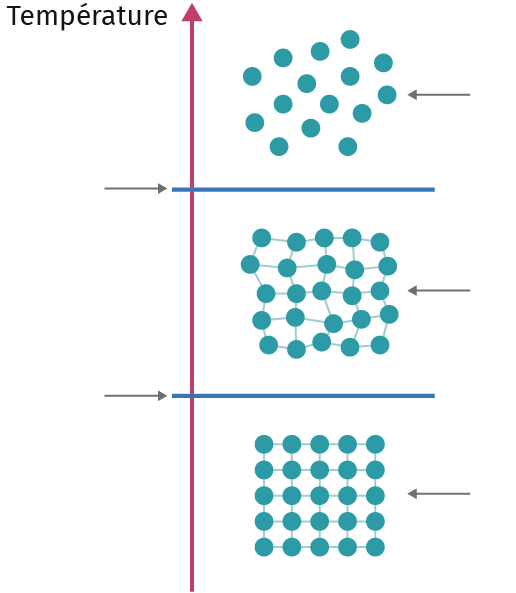
\includegraphics[width=0.6\linewidth]{evaluations/changement_etat.png}
\end{center}

\exo{Un fil de cuivre est :}{0}
\vspace*{-0.3cm}
\begin{qcm}
  \item Un corps pur.
  \item Un mélange.
  \item Une solution.
\end{qcm}
  % %%%% début de la page
\newpage
\enTete{Mouvement et interactions}{2}

\nomPrenomClasse

%%%% titre
\vspace{8pt}
\chevron L'objectif de cette interrogation \textbf{non notée} est d'évaluer où vous en êtes en physique-chimie.

%%%% question
%
\exo{Indiquer l'unité qui correspond à une vitesse.}{0}
\begin{qcm}
  \item Le mètre par seconde (m/s).
  \item Le kilomètre heure (km$\cdot$h).
  \item La seconde par mètre (s/m).
\end{qcm}

%
\exo{Une vitesse instantanée est représentée par une flèche qui porte 3 informations :}{0}
\begin{qcm}
  \item la distance, la direction et la durée.
  \item le sens, l'accélération et le nombre.
  \item la direction, le sens et la valeur.
\end{qcm}

%
\exo{Une observatrice observe depuis le quai un métro roulant à une vitesse constante.
Pour cette observatrice, le mouvement apparent du train est :}{1}

%
\exo{Un observateur est assis dans le métro roulant à une vitesse constante. 
Pour cet observateur, le mouvement apparent du train est :}{1}

%
\exo{Donner la formule de la force de pesanteur, le poids $P$, que l'on ressent sur Terre.}{1}

%
\exo{Indiquer la bonne expression de la force de pesanteur universelle $F_G$ entre deux objets de masse $m_A$ et $m_B$, séparés par une distance $d$.}{0}
\begin{qcm}
  \item $F_G = G \Frac{m_A m_B}{d^2}$
  \item $F_G = G m_A m_B$
  \item $F_G = G \Frac{m_A m_B}{d}$
\end{qcm}

%
\exo{Donner l'unité d'une force.}{1}
  
  %%%% Formative
  % %%%% début de la page
\newpage
\enTete{Corps purs et solutions}{1}

%%%%
\nomPrenomClasse

%%%% evaluation
\vspace*{6pt}
\begin{tableauCompetences}
  \centering RCO --
  Restituer ses connaissances.
  & & & &
  \\ \hline
  %
  \centering APP --
  Extraire une information
  & & & &
  \\ \hline
  %
  \centering REA --
  Réaliser un calcul.
  & & & &
\end{tableauCompetences}


%%%% questions
%
\exo{Un ensemble d'entités chimiques identiques est :\competence{RCO}}{0}
\vspace*{-4pt}
\begin{qcm}
  \item une espèce chimique.
  \item un corps pur.
  \item un mélange.
\end{qcm}

%
\exo{Définir un mélange.\competence{RCO}}{1}

%
\exo{Citer deux liquides \textbf{miscibles}.\competence{RCO}}{1}

%
L'acier doux est un alliage composé de fer (\chemfig{Fe}) et de carbone (\chemfig{C}).
Cet alliage est constitué d'une seule phase.
Un échantillon d'acier de masse $m = 1000 \unit{g}$ comporte une masse de fer $m_{\chemfig{Fe}} = 998 \unit{g}$ et une masse de carbone $m_{\chemfig{C}} = 2,\!00 \unit{g}$

%
\exo{Cet alliage est-il un mélange homogène ou hétérogène ?\competence{APP, RCO}}{1}

%
\exo{Écrire $m_{\chemfig{Fe}}$ et $m_{\chemfig{C}}$ en notation scientifique.\competence{APP, REA}}{1}

%
\exo{Calculer la proportion massique de fer et de carbone dans l'alliage.\competence{APP, REA}}{2}
  % %%%% début de la page
\newpage
\enTete{Corps purs et solutions}{1}

%%%%
\nomPrenomClasse

%%%% evaluation
\vspace*{6pt}
\begin{tableauCompetences}
  \centering RCO --
  Restituer ses connaissances.
  & & & & &
\end{tableauCompetences}


%%%% questions
%
\exo{Un ensemble d'entités chimiques identiques est : }{0}
\begin{qcm}
  \item une espèce chimique.
  \item un corps pur.
  \item un mélange.
\end{qcm}

%
\exo{Définir un mélange.}{1}

%
\vspace*{-12pt}
\exo{Deux liquides sont dits miscibles si ils}{0}
\begin{qcm}
  \item forment un mélange homogène.
  \item forment un mélange hétérogène.
\end{qcm}

%
\exo{Citer deux liquides \textbf{non-miscibles}.}{1}

%
\vspace*{-12pt}
\exo{Donner la formule de la masse volumique, en précisant le sens des symboles utilisés.}{3}

%
\vspace*{-12pt}
\exo{Une solution est :}{0}
\begin{qcm}
  \item Un mélange homogène.
  \item Un mélange hétérogène.
\end{qcm}

%
\exo{Donner le nom d'une solution dont le solvant est l'eau.}{1}

%
\vspace*{-12pt}
\exo{Donner la formule de la concentration massique, en précisant le sens des symboles utilisés.}{3}
  % %%%% début de la page
\newpage
\enTete{Mouvement et interactions}{2}

%%%%
\nomPrenom

%%%% evaluation
\vspace*{6pt}
\begin{tableauCompetences}
  \centering RCO 
  & Restituer ses connaissances.
  & & & &
\end{tableauCompetences}
\vspace*{8pt}

%%%% questions
%
\exo{Indiquer l'unité qui correspond à une vitesse.}{0}
\vspace*{-8pt}
\begin{qcm}
  \item Le mètre par seconde (m/s).
  \item Le kilomètre heure (km$\cdot$h).
\end{qcm}

%
\exo{Une vitesse est représenté par un vecteur qui porte 4 informations :}{0}
\vspace*{-8pt}
\begin{qcm}
  \item la position, la distance, la direction et la durée.
  \item le point, le sens, l'accélération et le nombre.
  \item le point d'application, la direction, le sens et la norme.
\end{qcm}

%
\exo{Une observatrice voit passer un métro roulant à une vitesse constante.
Pour elle le mouvement du métro est :}{1}

%
\exo{Un observateur est assis dans le métro roulant à une vitesse constante. 
Pour lui le mouvement du métro est :}{1}

%
\exo{Donner la formule du vecteur vitesse $\vv{v}_2$ d’un système au point $P_2$ entre les instants $t_1$ et $t_3$ :}{1}
  
  %%%% Fiche réussite
  % \enTeteFicheReussite{Chapitre 1 - Mélange et corps purs}

\begin{tableauConnaissancesSansExercices}
  Je sais la différence entre une espèce chimique et une entité chimique.
  & & & TP 1.1 \\
  % 
  Je sais la différence entre un corps pur et un mélange.
  & & & TP 1.1, TP 1.4 \\
  %
  Je sais décrire la composition d'un mélange avec les fractions volumiques et massiques.
  & & & activité 1.1 \\
  %
  Je connais la relation qui définit la masse volumique $\rho = m/V$.
  Je connais les unités et le sens de ces grandeurs. 
  Je sais calculer un volume, une masse ou une masse volumique avec cette relation.
  & & & TP 1.2, 1.3 et activité 1.2 \\
  %
  Je sais reconnaître si un échantillon est un corps pur constitué d'une seule espèce chimique ou s'il s'agit d'un mélange.
  & & & TP 1.1, TP 1.4, activité 1.1 \\
  %
  Je sais identifier un échantillon à partir de données physiques qui le caractérisent.
  & & & TP 1.2, TP 1.3 \\
  %
  Je sais identifier une espèce chimique à partir de tests chimiques caractéristiques.
  & & & TP 1.3 \\
  %
  Je connais le vocabulaire de la chromatographie sur couche mince : ligne de dépôt, couche mince, éluant, front de l'éluant, etc.
  & & & TP 1.4 \\
  % 
  Je sais analyser un chromatogramme pour identifier des espèces chimiques.
  & & & TP 1.4 \\
  % 
  Je sais analyser un chromatogramme pour reconnaitre un corps pur d'un mélange.
  & & & TP 1.4 \\
\end{tableauConnaissancesSansExercices}


\basDePageFicheReussite

\questionFicheReussite{3}

  % \enTeteFicheReussite{Chapitre 1 - Solutions}
\bigskip

\begin{tableauConnaissances}
  Je sais qu'une solution est un mélange homogène.
  Je sais qu'une solution est composé d'un solvant, l'espèce chimique majoritaire, et de un ou plusieurs solutés.
  & & & TP 4, cours p. 9 & 11 p. 48 \\
  %
  Je sais qu'on parle de solution aqueuse quand le solvant est l'eau.
  & & & TP 4 \& 5, cours p. 9 & \\
  %
  Je connais la formule de la concentration massique $c = m/V$.
  Je connais les unités et le sens de ces grandeurs.
  Je sais calculer une concentration massique, une masse ou un volume avec la formule.
  & & & TP 4 \& 5, cours p. 9, 10 & 14, 15 p. 49 \\
  %
  Je sais ce qu'est une dilution et une dissolution.
  Je connais le protocole pour réaliser une dilution.
  & & & TP 1, 4 \& 5, cours p. 10, 11 & 12, 16 p. 49 \\
  %
  Je sais qu'un dosage est une mesure de concentration.
  Je sais réaliser un dosage par étalonnage, en mesurant une grandeur proportionnelle à la concentration.
  & & & TP 4 \& 5, cours p. 12 & \\
\end{tableauConnaissances}

\basDePageFicheReussite{3}
  % \enTeteFicheReussite{Chapitre 2 - \sndChapitreDeux}
\bigskip

\begin{tableauConnaissances}
  % 
  Je sais que le mouvement dépend du référentiel choisi et je connais le modèle du point matériel.
  & & & Activité 1, 2 \& 3, cours p. 1-4 & 11, 13 p. 210
  \\ \hline 
  %
  Je sais décrire le mouvement d'un système (trajectoire + évolution de son vecteur vitesse). Je sais reconnaitre un mouvement rectiligne uniforme.
  & & &  Activité 1, 2 \& 3, cours p. 1-4 & 11, 14 p.210-211
  \\ \hline
  %
  Je sais calculer et tracer un vecteur vitesse à partir du vecteur déplacement et de l'écart de temps entre deux positions. 
  & & & Activité 3 \& 7, cours p. 1-4 & 14, 16 p. 211, 11 p. 243
  \\ \hline
  %
  Je sais qu'une force s'exprime en newton (N) et je sais représenter une force en terme de vecteurs, en faisant attention à son point d'application.
  & & & Activité 4 \& 5, cours p. 6-8 & 15, 16 p. 228, 10 p. 243 
  \\ \hline
  %
  Je connais les caractéristiques des forces suivantes : poids, réaction du support et forces de frottements.
  & & & Activité 4 \& 5, cours p. 6-8 & 11, 14, 17 p. 227-228
  \\ \hline
  %
  Je sais utiliser le principe d'inertie et sa contraposée pour relier le mouvement d'un système au forces qui s'exercent sur lui.
  & & & Activité 5, 6, 7 \& 8, cours p. 9-10 & 10, 11 p.243
  %
\end{tableauConnaissances}

\basDePageFicheReussite{2}
  % \enTeteFicheReussite{Chapitre 3 - Atome et ordre de grandeur}
\bigskip

\begin{tableauConnaissances}
  % 
  Je sais calculer et utiliser les puissances de dix.
  Je sais utiliser la notation scientifique.
  Je sais calculer un ordre de grandeur avec les puissances de dix.
  & & &  Activité 1 & Exercice 15, 16 \& 27 p. 81
  \\ \hline
  %
  Je sais que la masse d’un atome est essentiellement contenue dans celle de son noyau.
  Je sais que le noyau est très petit devant la taille de l'atome.
  & & & Activité 2 & Exercice 9, 13 p. 81
  \\ \hline
  %
  Je connais les charges électriques des électrons, neutrons et protons.
  J'ai compris pourquoi l'atome a une charge globale neutre.
  & & & Activité 2 \& 3 &
  \\ \hline
  %
  Je connais les composants d'un atome et de son noyau. 
  Je sais faire la différence entre électrons, protons, neutrons et nucléons.
  & & & Activité 3 &
  \\ \hline
  %
  Je peux déterminer la composition d'un atome à partir de sa notation symbolique \isotope{A}{Z}{X} et inversement.
  & & & Activité 3 & Exercice 7, 13 p. 81 
  \\ \hline
  %
  Je sais faire la différence entre les termes atome, ion, isotope.
  & & & Activité 3 & 
  \\ \hline
  %
  Je sais que la description d'un atome est un modèle, dont l'évolution dépend d'observations expérimentales.
  & & & Activité 4 & Doc. p. 105
  %
\end{tableauConnaissances}

\basDePageFicheReussite
\bigskip

\coursFicheReussite
  % \enTeteFicheReussite{Chapitre 3 - Cortège électronique, ions, molécules}
\bigskip

\begin{tableauConnaissances}
  %
  %Je sais que les électrons se structurent en couche (1, 2, 3) et sous-couche (s, p) autour du noyau.
  Je peux écrire la configuration électronique d'un atome en remplissant les sous-couches s et p dans le bon ordre.
  & & & Activité 5, 6 &
  \\ \hline
  %
  Je sais que les éléments chimiques sont rangées par colonne (famille) et par ligne (période) dans le tableau périodique.
  & & & Activité 6 &
  \\ \hline
  %
  Je peux identifier la couche externe d'un atome et combien d'électrons de valence s'y trouvent.
  & & & Activité 5, 6, 7, 8 &
  \\ \hline
  %
  Je sais repérer la famille des gaz nobles dans le tableau périodique.
  Je sais que leur couche externe pleine les rend très stables.
  & & & Activité 6, 7, 8 &
  \\ \hline
  %
  Je connais la règle du duet et de l'octet.
  Je peux les appliquer pour trouver quel ion stable peut être formé à partir d'un atome.
  & & & Activité 7 &
  \\ \hline
  %
  Je sais que les molécules sont composées d'atomes.
  Je sais que la stabilité d'une molécule est due aux électrons de valence partagés entre les atomes.
  & & & Activité 8 &
  \\ \hline
  %
  Je peux analyser un schéma de Lewis pour expliquer la stabilité d'une molécule.
  & & & Activité 8 &
  \\ \hline
  %
  Je sais qu'une espèce chimique est constitué d'un très grand nombre d'entités chimiques.
  Je sais ce que représente une mole.
  & & & Activité 9 &
  %
  %
\end{tableauConnaissances}

\basDePageFicheReussite
\bigskip

\coursFicheReussite
  % \enTeteFicheReussite{Chapitre 4 - Ondes lumineuses et optique}
\bigskip

\begin{tableauConnaissancesSansExercices}
  %
  Je sais que la lumière est une onde électromagnétique.
  Je sais que la lumière peut être monochromatique ou polychromatique.
  & & & Activité 1
  \\ \hline
  %
  Je connais les deux types de spectre d'émission et je sais les reconnaître.
  & & & TP 1
  \\ \hline
  %
  Je sais qu'un corps chaud produit un spectre continu.
  Les propriétés de ce spectre dépendent de la température du corps chaud.
  & & & TP 1
  \\ \hline
  %
  Je sais qu'un gaz atomique ou moléculaire excité produit un spectre de raies.
  Je sais que chaque élément chimique possède son propre spectre de raies qui permet de le reconnaître.
  & & & TP 1, activité 2
  \\ \hline
  %
  Je sais repérer une raie sur un spectre en mesurant sa longueur d'onde.
  & & & TP 1, activité 2
  \\ \hline
  %
  Je connais le vocabulaire de la réfraction et je sais lire les angles d'incidence et de réfraction à partir d'un schéma.
  & & & TP 2, activité 4
  \\ \hline
  %
  Je sais appliquer la loi de Snell-Descartes pour calculer un indice de réfraction ou un angle.
  & & & TP 2, activité 4
  \\ \hline
  %
  Je sais expliquer comment l'oeil parvient à faire l'image d'un objet.
  & & & Activité 3
  \\ \hline
  %
  Je sais expliquer comment fonctionne une lentille convergente et je connais le vocabulaire pour la décrire (foyer image, foyer objet, centre optique).
  & & & TP 3, activité 3
  \\ \hline
  %
  Je connais la formule du grandissement et je sais l'appliquer pour calculer la taille d'un objet ou d'une image.
  & & & TP 3, Activité 3
  \\ \hline
  %
  Je sais expliquer pourquoi la lumière blanche est dispersée après avoir traversé un prisme.
  & & & Activité 4
  %
\end{tableauConnaissancesSansExercices}
\bigskip 

% \basDePageFicheReussite
% \coursFicheReussite
\questionFicheReussite{2}

  %%%%%%%% Terminale
  %%%% Formative
  % \teteTermStssOrga

\begin{center}
  \chemfig{
    HO- C (=[3] O) -CH (-[-3] NH_2) -CH_3
  }
  \\[8pt]
  \important{Alanine}, un acide aminé
\end{center}

\question{
  Donner le nom de la formule utilisée pour représenter la molécule d'alanine.
}{
  C'est la formule semi-developpée.
}{1}

\question{
  Donner la formule brute de l'alanine.
}{
  \chemfig{C_3 H_7 O_2 N}
}{1}

\question{
  Donner la formule développée de l'alanine.
}{
  \chemfig{
    H-O- C (=[3] O) -C (-[3] H) (-[-3] N (-[-5]H) (-[-1] H)) -C (-[3] H) (-[-3] H) -H
  }
}{6}
  
\numeroQuestion
Entourer deux groupe fonctionnels dans la molécule d'alanine et les nommer.
  % \teteTermStssOrga
\nomPrenom

\begin{center}
  \chemfig{
    [:150]
    *6(-=-=-=) % phenyl
    -[0]-[-2]
      (-[-4] (=[6]O) -[-2]O -[-4]) % ester
    -[0]NH -[-2,,1] (=[-4] O) % Amide
    -[0] (-[2] NH_2) % amine
    -[-2] -[0] (=[2] O) -[-2] OH % acide carboxylique
  }
  \\[8pt]
  \important{Aspartame}, molécule au gout sucré
\end{center}

\question{
  Donner le nom de la représentation de la molécule d'aspartame
}{
  C'est la formule topologique.
}{1}

\question{
  Donner la formule brute de l'aspartame.
}{
  \chemfig{C_{14} H_{18} N_{2} O_{5}}
}{1}

\question{
  Entourer les quatre groupes fonctionnels dans la molécule d'aspartame et les nommer.
}{
  Ester, amide, amine et acide carboxylique
}{4}
  % \teteTermStssOrga

\begin{center}
  \chemfig{
    HO-[1] *6(-- % 1er cycle
      *6(=-- % 2eme cycle
        *6(- % 3eme cycle
          *5(--- 
            (-[:60] (-[:120]) -[:10] -[:60] -[:10] -[:60] (-[:120]) -[:10]) % lipide
          - (-[:90]) -) % 4eme
        ----) % 3eme
      ---) % 2eme
    - (-[:90]) ---) % 1er
  }
  \\[8pt]
  \important{Cholestérol}, lipide de la famille des stérol
\end{center}

\question{
  Donner le nom de la représentation de la molécule.
}{
  C'est la formule topologique.
}{1}

\question{
  Donner la formule brute du cholestérol.
}{
  \bruteCHO{27}{42}
}{1}

\question{
  Entourer et nommer le(s) groupe(s) fonctionnel(s) du cholestérol.
}{
  Alcool et alcène.
}{2}

%\vfill 
%Si on devait utiliser la nomenclature pour nommer la molécule de cholestérol, son nom serait

% \centering
% (3S, 8S, 9S, 10R, 13R, 14S, 17R)-10,13-diméthyl-17-[(2R)-6-méthylheptan-2-yl]-2,3,4,7,8,9,11,12,14,15,16,17-dodécahydro-1H-cyclopenta[a]phénanthren-3-ol
  % \teteTermStssOrga

\nomPrenom

\begin{center}
  \chemfig{
    *6 (-(-OH) -(-OH) -(-OH) -O -(- -[3]OH) -) (-[-5]HO)
  }
\end{center}

\question{
  Donner la formule brute de cette molécule.
}{
  \bruteCHO{6}{12}{6}
}{1}

\question{
  Donner le nom de cette molécule.
}{
  Le glucose
}{1}

\question{
  Entourer les groupes caractéristiques de la molécule et les nommer.
}{
  Alcool et ether.
}{4}
  
  %%%% Compétences
  % %\newpage
\pasDePagination

%%%% liste des compétences
\titre{Liste des compétences évaluées}

Ce tableau liste l'ensemble des compétences évaluées au cours de l'année.
Ces compétences sont liées à la méthode scientifique : chaque compétence représente une étape nécessaire pour étudier une situation nouvelle en appliquant la méthode scientifique.
Pour chaque compétence, des exemples de capacités concrètes sont présentées.
\bigskip

L'objectif de cette liste est de vous aider à identifier ce qui est attendu de vous au cours de l'année.
\bigskip

Au début de chaque évaluation, les compétences effectivement évaluées seront présentées clairement. 
\bigskip

\begin{tabularx}{\linewidth}{| m{0.2\linewidth} | X |}
  \hline
  \rowcolor{gray!20} 
  \centering \textbf{Compétences} & \textbf{Capacités associées}
  \\ \hline
  %
  \centering Restituer ses connaissances (RCO) &
  -- Énoncer les définitions du cours. \newline
  -- Énoncer des exemples courants présentés en cours
  \\ \hline
  %
  \centering S'approprier (APP) &
  -- Énoncer un problème à résoudre (problématique). \newline
  -- Rechercher et organiser l'information. \newline
  -- Représenter la situation par un schéma.
  \\ \hline
  %
  \centering Analyser/ Raisonner (ANA/RAI) &
  -- Formuler des hypothèses. \newline
  -- Proposer une stratégie de résolution. \newline
  -- Évaluer des ordres de grandeurs. \newline
  -- Choisir un modèle ou des lois pertinentes. \newline
  -- Choisir, élaborer, justifier un protocole. \newline
  -- Prévoir à l'aide d'un modèle. \newline
  -- Procéder à des analogies.
  \\ \hline
  %
  \centering Réaliser (REA) &
  -- Mettre en \oe{}uvre les étapes d'une démarche. \newline
  -- Utiliser un modèle. \newline
  -- Calculer, représenter, collecter des données, etc. \newline
  -- Mettre en \oe{}uvre un protocole expérimental en respectant les règles de sécurités.
  \\ \hline
  %
  \centering Valider (VAL) & 
  -- Faire preuve d'esprit critique. \newline
  -- Identifier des sources d'erreur, estimer une incertitude .\newline
  -- Comparer avec des valeurs de références. \newline
  -- Confronter un modèle à des résultats expérimentaux. \newline
  -- Proposer des améliorations de la démarche ou du modèle.
  \\ \hline
  %
  \centering Communiquer (COM) &
  -- Présenter de manière argumentée, synthétique et cohérente. \newline
  -- Utiliser un vocabulaire ou une représentation adaptée. \newline
  -- Échanger entre élèves.
  \\ \hline
\end{tabularx}
  % \newcommand{\competenceClasseur}{
  \begin{center}
    \setlength{\extrarowheight}{6pt}
    \begin{tabular}{| l | c | c | c | c |}
      \hline
      \rowcolor{gray!20} 
      %
      \textbf{Items évalués} & D & C & B & A
      \\ \hline
      %
      Propreté  & & & &
      \\ \hline
      %
      Rangement (feuilles dans le bon ordre) & & & &
      \\ \hline
      %
      Complétion (feuilles présentes \textit{et} remplies) & & & & 
      \\ \hline
    \end{tabular}
  \end{center}
}

\pasDePagination

\competenceClasseur
\bigskip
\competenceClasseur
\bigskip
\competenceClasseur
\bigskip
\competenceClasseur
\bigskip
\competenceClasseur
\end{document}